%%%%%%%%%%%%%%%%%%%%%%%%%%%%%%%%%%%%%
% CHAPTER 3: Experimental Procedure %
%%%%%%%%%%%%%%%%%%%%%%%%%%%%%%%%%%%%%
%................................
% Notes about things to add/edit 
%................................
% >> Determine best way to present the Fig+Table combinations
% >> Add test matrix
% 		* Items: Test Name, Structure, Description 
% 		* Potential additions: ramp or instant? Multiple seqs? PPV? 
% 				Duration? Variation of parameters? Ambient Temp?
% 				Open Vents?
% >> Text alignment after double digit numbers in event time tables
%%%%%%%%%%%%%%%%%%%%%%%%%%%%%%%%%%%%%%%%%%%%%%%%%%%%%%%%%%%%%%%%%%%%%

\renewcommand{\thechapter}{3}

\chapter{Experimental Procedure}
\label{chap:exp_procedure}

A similar procedure was followed for all nine propane gas burner experiments described in this report. First, the three propane burners were ignited in sequential order. Next, various doors and vents were opened and closed to change the ventilation pattern in the structure. Then, the burners were turned off, extinguishing the fire. After the burners were extinguished, data continued to be collected while different doors and vents were opened to cool the interior of the structure. A positive pressure ventilation (PPV) fan was used during some tests to expedite the cooling of the structure. 

The nine propane gas burner tests were conducted in series with a variety of other experiments. In order to be consistent with the original test numbering, the gas burner experiments described in this report are referred to as Tests~2--6 and Tests~22--25. The experiments and their different parameters are summarized in Table~\ref{table:exp_summary} below.

\renewcommand{\baselinestretch}{1}
\begin{sidewaystable}[!ht]
\begin{center}
\caption{Summary of Propane Gas Burner Experiments.}
\begin{tabular}{ccccl}
\toprule
% \multirow{2}{*}{Test~\#}    
\textbf{Name}  	& 	\textbf{Structure} 	& 	\textbf{Duration of Fire} 	& 	\textbf{Heat Release Rate} 	& 	\multicolumn{1}{c}{\textbf{Ventilation}}	\\ 
				& 						& 		\textbf{(min:sec)} 		& 	\textbf{Rate (kW)}			& 													\\
\midrule
Test 2 			& 	East 				&  		16:01 					& 	N.R.$^*$ 					& 	Both double doors, south door, PPV after fire	\\
Test 3			& 	East 				&  		16:58 					&   N.R.$^*$   					& 	Both double doors, south door, PPV after fire					\\
Test 4			& 	East 				&  		16:59 					&  	N.R.$^*$ 					& 	Both double doors, south door, PPV after fire					\\
\multicolumn{5}{c}{} \\
Test 5 			& 	East 				&  		 9:36 					&  		1190 					& 	Roof vent, both double doors				 					\\
				& 						& 		10:15 					&  		1190 					& 	Roof vent, both double doors				 					\\
				& 						& 		 9:32 					&  		1190 					& 	Roof vent, both double doors				 					\\				
\multicolumn{5}{c}{} \\
Test 6			&	East 				&  		 5:27 					&  		1190 					& 	Roof vent, west double door					 	    			\\
				& 						& 		 5:03 					&  		1190 					& 	Roof vent, west double door					 	    			\\
				& 						& 		 5:12 					&  		1180 					& 	Roof vent, west double door					 	    			\\
\multicolumn{5}{c}{} \\
Test 22			&	West 				&  		16:58 					&  		1240 					& 	Both sets of double doors, 2nd floor south door, PPV fan 		\\
Test 23			&	West 				&  		16:58 					&  		1290 					& 	Both sets of double doors, PPV fan						 		\\
Test 24			&	West 				&  		16:58 					&  		1270 					&   West double door on both floors, 2nd floor south door, PPV fan 	\\
Test 25			&	West 				&  		16:58 					&  		1270 					& 	West double door on both floors, 2nd floor south door, PPV fan 	\\
\bottomrule
\multicolumn{5}{l}{$^*$\footnotesize{Not reported because propane flow rate was not accurately measured during tests}}
\end{tabular}
\end{center}
% $^1$ \footnotesize Not reported because propane flow rate could not be accurately measured during tests
\label{table:exp_summary}
\end{sidewaystable}
\clearpage
% FloatBarrier

\section{East Structure Tests}
Five different tests, Tests~2--6, were conducted in the East Structure. Table~\ref{table:HRR_Tests_5-6} lists the heat release rates for Tests~5 and 6. The time between the ignition of each gas burner for Tests~5 and 6 was on the order of seconds. As a result, a single heat release rate, one for all three burners ignited, is reported.

\renewcommand{\baselinestretch}{1}
% \begin{table}[h]
% \caption[Heat Release Rates for Tests~5 and 6.]{Heat Release Rates (kW) for Tests~5 and 6.}
% \begin{center}
% \begin{tabular}{|c|c|}
% \hline
%  % & \textbf{Heat Release Rate (kW)} \\
% \multirow{2}{*}{Test~\#}    & Heat Release Rate for \\ 
% 							& all Burners Ignited (kW) \\
% \hline \hline
% 5 -- Seq. 1		& 1190 \\
% 5 -- Seq. 2		& 1190 \\
% 5 -- Seq. 3		& 1190 \\
% 6 -- Seq. 1		& 1190 \\
% 6 -- Seq. 2		& 1190 \\
% 6 -- Seq. 3		& 1180 \\
% \hline
% \end{tabular}
% \end{center}
% \label{table:HRR_Tests_5-6}
% \end{table}

\begin{table}[!ht]
\caption[Heat Release Rates for Tests~5 and 6.]{Heat Release Rates for Tests~5 and 6.}
\begin{center}
\begin{tabular}{lc}
 \toprule
 & \textbf{Heat Release Rate (kW)} \\
\textbf{Test} & \textbf{All Burners On} \\
\midrule
Test 5 - Seq. 1		& 1190 \\
Test 5 - Seq. 2		& 1190 \\
Test 5 - Seq. 3		& 1190 \\
Test 6 - Seq. 1		& 1190 \\
Test 6 - Seq. 2		& 1190 \\
Test 6 - Seq. 3		& 1180 \\
\bottomrule
\end{tabular}
\end{center}
\label{table:HRR_Tests_5-6}
\end{table}
\FloatBarrier

\subsection{Tests 2--4}
Tests~2--4 followed a nearly identical order of events. Figure~\ref{fig:Tests_2-4_layout} includes a schematic floor plan and table of event times corresponding to the data files for each test. A 0.61~cm (2.0~ft) diameter PPV fan located 1.6~m (5.2~ft) away from the south exterior door was aimed at the center of the doorway and used after all burners were extinguished. During Tests~2--4, the south exterior door was not able to completely close due to an obstruction caused by the hoses used to transport the propane to the burners. So, when the south door was in the ``closed'' position, a 133~mm (5.25~in) opening was present between the door and its frame. For all other experiments, however, the south exterior door was not used and the doorway remained closed for the entirety of the test. To fully close the doorway during these tests, the hinged door was removed and replaced by a piece of gypsum board that completely covered the doorway.
\\
\begin{figure}[!ht]
\renewcommand{\baselinestretch}{1}
\begin{minipage}[b]{1.01\columnwidth}
\begin{center}
	% \begin{flushleft}
	\begin{tabular}{lccc}
	\multicolumn{4}{c}{\normalsize Event Times (sec) for Tests~2--4 Data Files} \\
	\toprule
	\multicolumn{1}{c}{\textbf{Event}} 	& \textbf{Test 2} & \textbf{Test 3} & \textbf{Test 4} \\
	\midrule
	~(1)~ Corner burner on 				& 	0		  	  &	 	0			&		0		  \\
	~(2)~ Middle burner on 				&   181			  &		181			&		179		  \\
	~(3)~ Center burner on 				&   361			  &	   	361			&	   	360		  \\
	~(4)~ West double door opened 		&   418			  &    	416			&	   	415		  \\
	~(5)~ East double door opened 		&   538			  &    	536			&	   	535		  \\
	~(6)~ South exterior door opened 	&   604			  &    	597			&	   	597		  \\
	~(7)~ Center burner off				&   720			  &    	778			&	   	778		  \\
	~(8)~ Middle burner off				&   840			  &    	898			&	   	897		  \\
	~(9)~ Corner burner off				&   961			  &    	1018		&	   	1019	  \\
	(10) PPV fan on 					& 	1256		  &    	1316		&  	   	1319	  \\
	(11) PPV fan off 					& 	1892 		  & 	N/A 		& 		1380	  \\
	(12) PPV fan on 					& 	N/A 		  & 	N/A 		& 		1487 	  \\
	\bottomrule
	\end{tabular}
	% \end{flushleft}
	% \begin{tabular}{|l|c|c|c|}
	% \multicolumn{4}{c}{Event Times (sec) for Tests~2--4 Data Files}
	% \vspace{5pt} \\
	% \hline
	% \multicolumn{1}{|c|}{Event}		    & Test 2 		  & Test 3 			& Test 4 \\
	% \hline \hline
	% ~(1)~ Corner burner on 				& 	0		  	  &	 	0			&		0		  \\
	% ~(2)~ Middle burner on 				&   181			  &		181			&		179		  \\
	% ~(3)~ Center burner on 				&   361			  &	   	361			&	   	360		  \\
	% ~(4)~ West double door opened 		&   418			  &    	416			&	   	415		  \\
	% ~(5)~ East double door opened 		&   538			  &    	536			&	   	535		  \\
	% ~(6)~ South exterior door opened 	&   604			  &    	597			&	   	597		  \\
	% ~(7)~ Center burner off				&   720			  &    	778			&	   	778		  \\
	% ~(8)~ Middle burner off				&   840			  &    	898			&	   	897		  \\
	% ~(9)~ Corner burner off				&   961			  &    	1018		&	   	1019	  \\
	% (10) PPV fan on 					& 	1256		  &    	1316		&  	   	1319	  \\
	% (11) PPV fan off 					& 	1892 		  & 	N/A 		& 		1380	  \\
	% (12) PPV fan on 					& 	N/A 		  & 	N/A 		& 		1487 	  \\
	% \hline
	% \end{tabular}
\end{center}
\end{minipage}
\begin{minipage}[b]{0.9\columnwidth}
	\vspace{20pt}
	\centering
	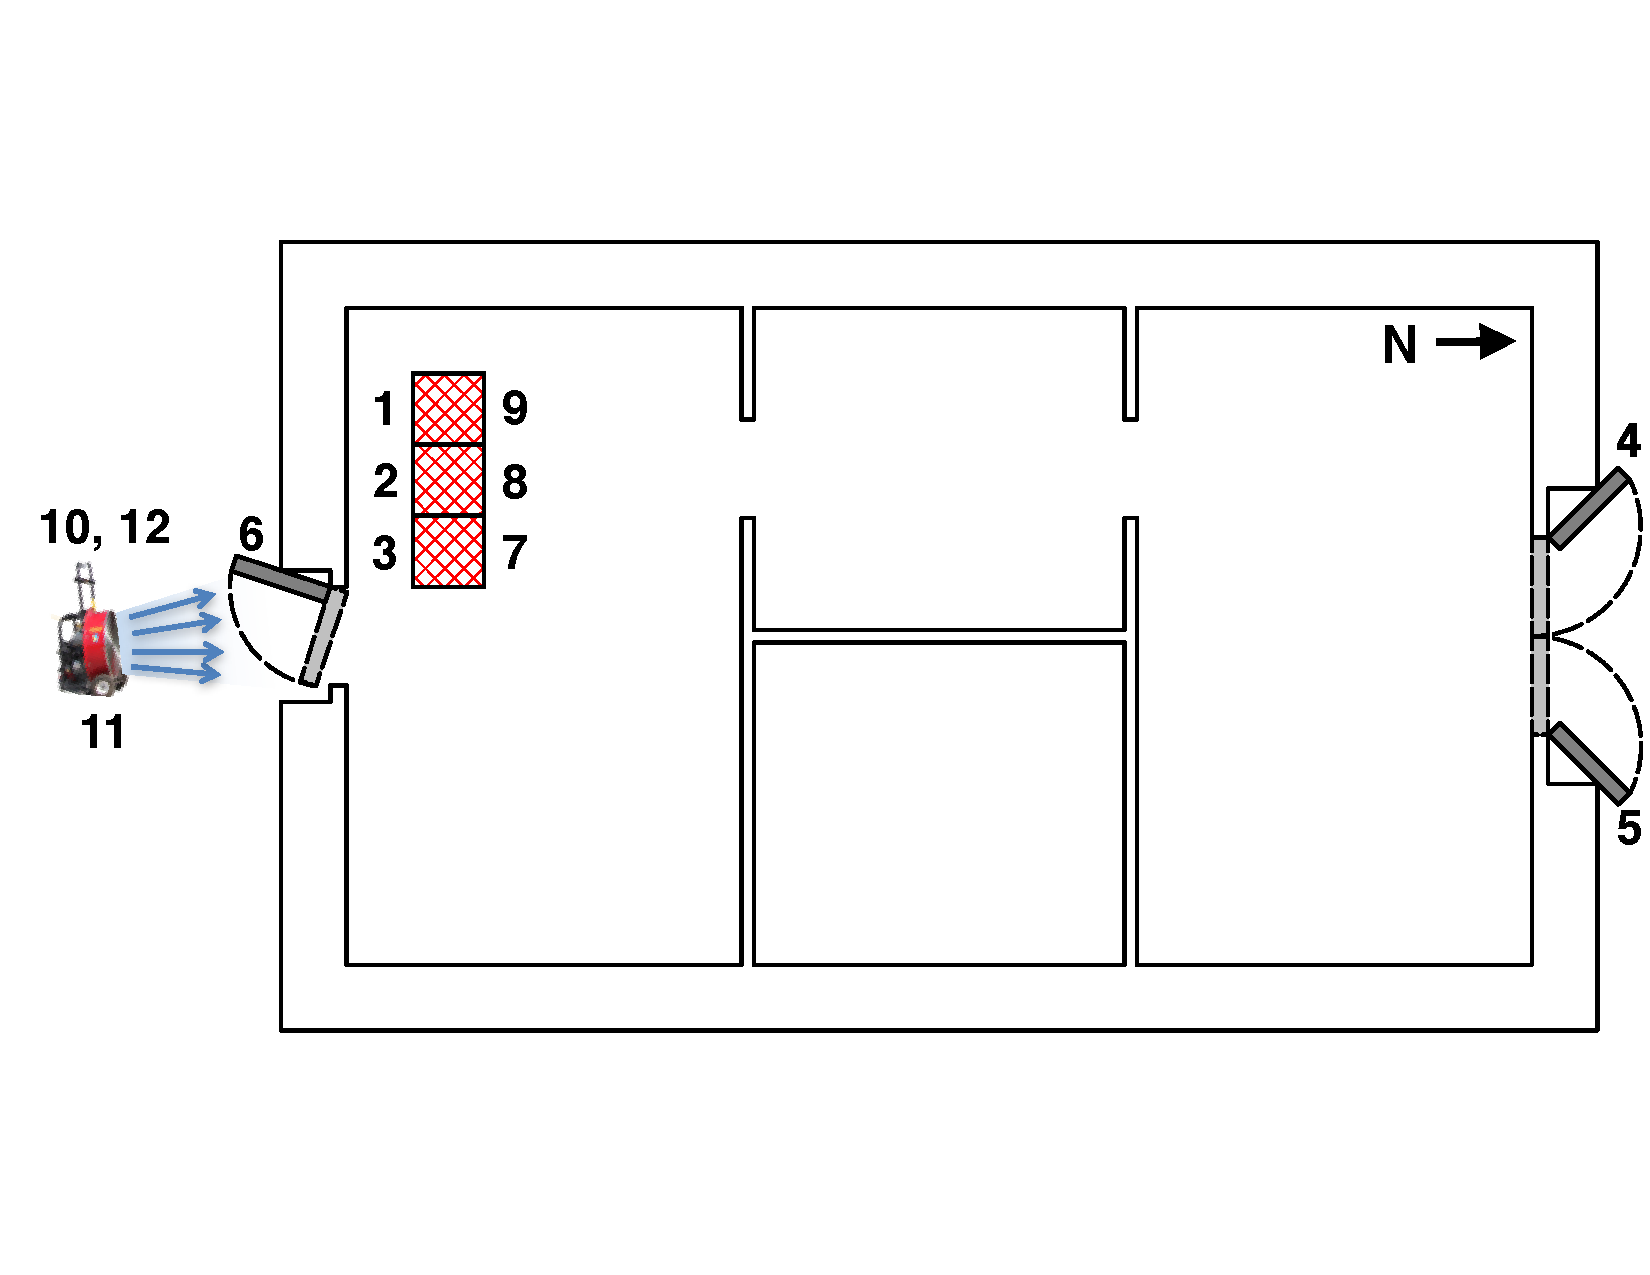
\includegraphics[width=\columnwidth]{Figures/Floor_Plans/East_Structure_Test_4}
\end{minipage}
\renewcommand{\baselinestretch}{1}
\caption{Tests~2--4 layout and event times.}
\label{fig:Tests_2-4_layout}
\end{figure}
\FloatBarrier

\subsection{Tests 5 \& 6}
The procedures for Tests~5 and 6 are outlined in Figures~\ref{fig:east_test_5} and \ref{fig:east_test_6}, respectively. Both tests involved repeating a specific set of events three times in a row. To avoid listing the identical actions three separate times in the ``event'' column of the tables, each repetition of events is denoted as a ``sequence'' (abbreviated as ``seq.''), and each table contains three columns of times --- one for each sequence.
\\
% \begin{figure}[!ht]
% \begin{minipage}[b]{0.8\columnwidth}
% 	\begin{flushleft}
% 	\begin{tabular}{lccc}
% 	\multicolumn{4}{c}{\normalsize Event Times (s) for Test~5 Data File} \\
% 	\toprule
% 	\multicolumn{1}{c}{\textbf{Event}} 	& \textbf{Seq. 1} & \textbf{Seq. 2} & \textbf{Seq. 3} \\
% 	\midrule
% 	~(1)~ All burners on 				& 	0			  &	   1225			&	   2425		\\
% 	~(2)~ Roof vent opened 				&   154			  &    1345			&	   2545		\\
% 	~(3)~ West double door opened 		&	175			  &	   1432	 		&	   2632 	\\
% 	~(4)~ East double door opened 		&   361			  &    1524			&	   2730		\\
% 	~(5)~ Roof vent closed		 		&   445			  &    1723			&	   2852		\\
% 	~(6)~ All burners off 				&   576			  &    1840			&	   2997		\\
% 	~(7)~ Roof vent opened				& 	720 		  &	   1890			&	   3086		\\
% 	~(8)~ East double door closed		& 	1148 		  &	   2311			&	   N/A		\\
% 	~(9)~ West double door closed		& 	1164 		  &	   2330			&	   N/A		\\
% 	(10) Roof vent closed		 		&   1179		  &    2387			&	   N/A		\\
% 	\bottomrule
% 	\end{tabular}
% 	\end{flushleft}
% \end{minipage}
% \begin{minipage}[b]{0.9\columnwidth}
% 	\vspace{15pt}
% 	\centering
% 	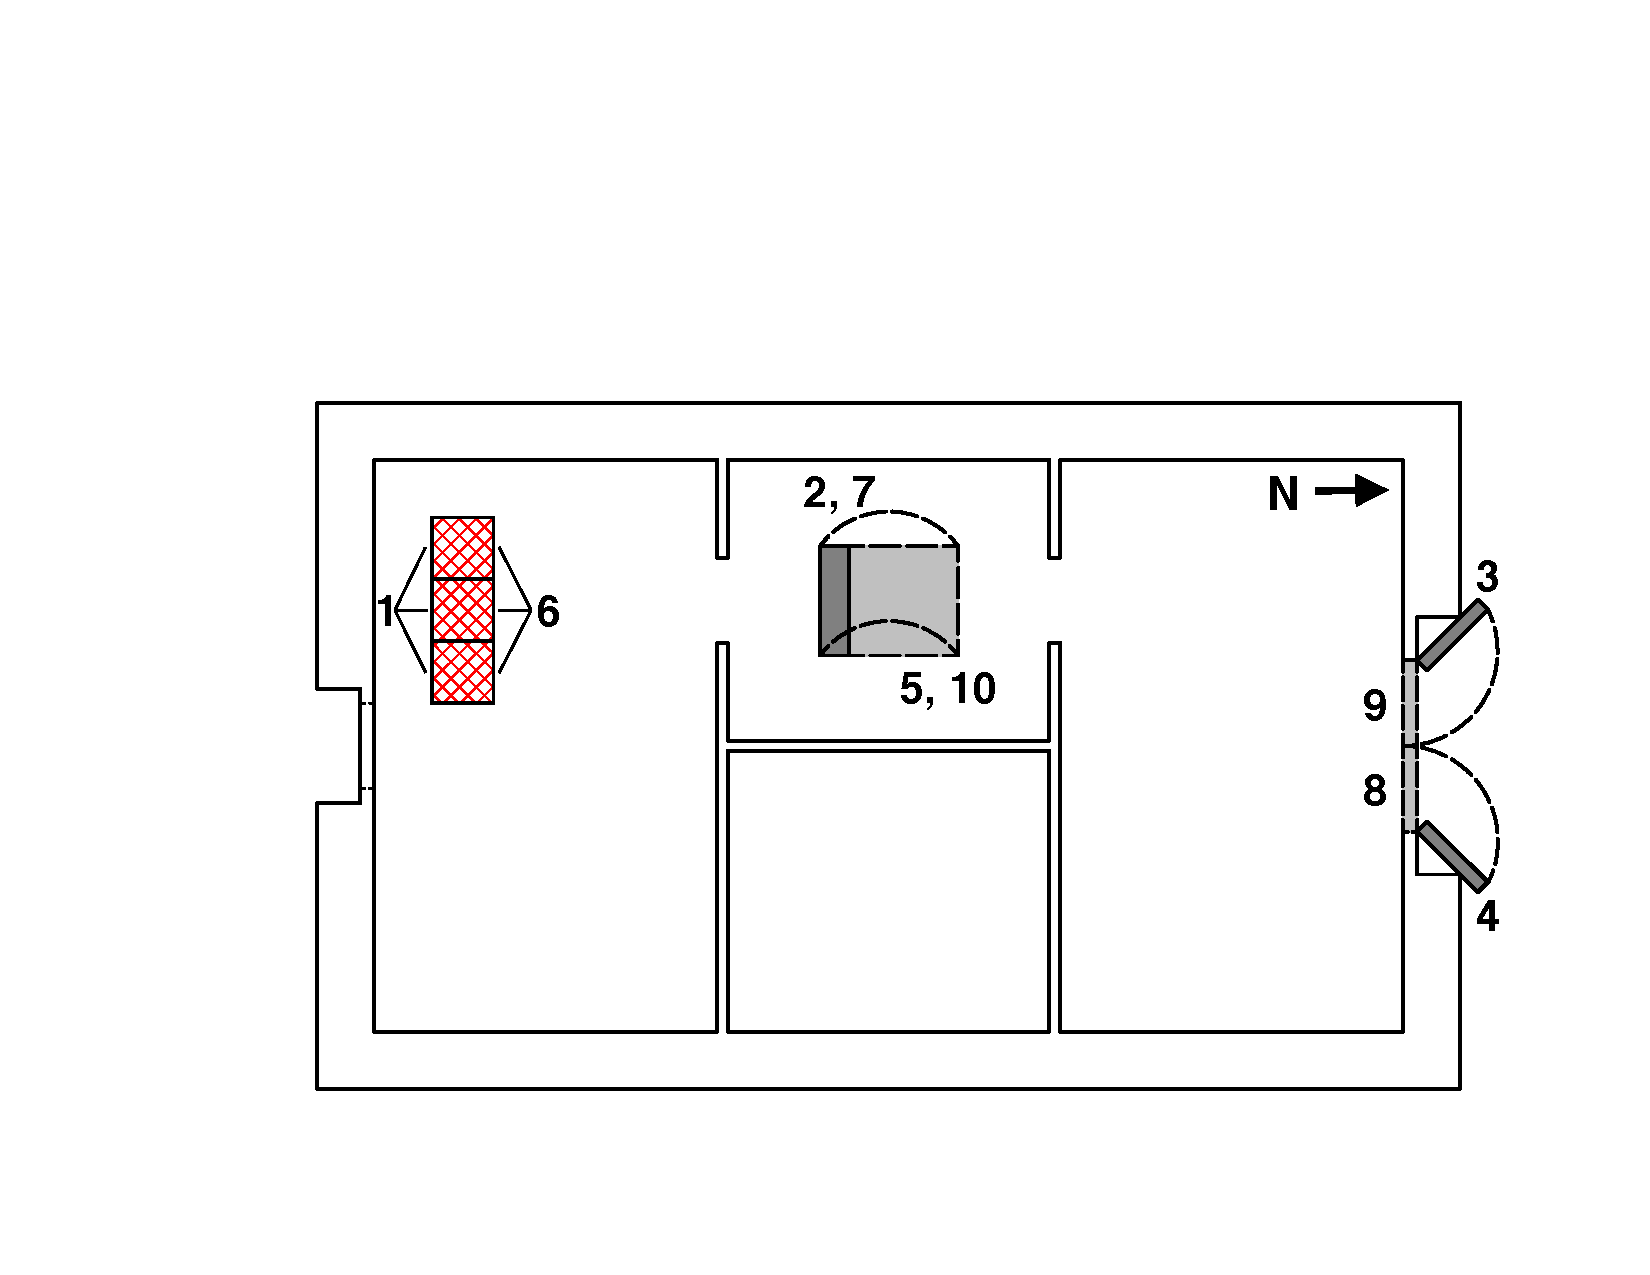
\includegraphics[width=0.86\columnwidth]{Figures/Floor_Plans/East_Structure_Test_5}
% \end{minipage}
% \caption{Test~5 layout and event times.}
% \label{fig:east_test_5}
% \end{figure}
% \clearpage

\begin{figure}[!ht]
\renewcommand{\baselinestretch}{1}
\begin{minipage}[b]{0.96\columnwidth}
\begin{center}
	\begin{tabular}{lccc}
	\multicolumn{4}{c}{\normalsize Event Times (sec) for Test~5 Data File} \\
	\toprule
	\multicolumn{1}{c}{\textbf{Event}} 	& \textbf{Seq. 1} & \textbf{Seq. 2} & \textbf{Seq. 3} \\
	\midrule
	~(1)~ All burners on 				& 	0			  &	   1225			&	   2425		\\
	~(2)~ Roof vent opened 				&   154			  &    1345			&	   2545		\\
	~(3)~ West double door opened 		&	175			  &	   1432	 		&	   2632 	\\
	~(4)~ East double door opened 		&   361			  &    1524			&	   2730		\\
	~(5)~ Roof vent closed		 		&   445			  &    1723			&	   2852		\\
	~(6)~ All burners off 				&   576			  &    1840			&	   2997		\\
	~(7)~ Roof vent opened				& 	720 		  &	   1890			&	   3086		\\
	~(8)~ East double door closed		& 	1148 		  &	   2311			&	   N/A		\\
	~(9)~ West double door closed		& 	1164 		  &	   2330			&	   N/A		\\
	(10) Roof vent closed		 		&   1179		  &    2387			&	   N/A		\\
	\bottomrule
	\end{tabular}
	% \begin{tabular}{|l|c|c|c|}
	% \multicolumn{4}{c}{Event Times (sec) for Test~5 Data File}
	% \vspace{5pt} \\
	% \hline
	% \multicolumn{1}{|c|}{Event}		    & Seq. 1 		  & Seq. 2 			& 	Seq. 3 \\
	% \hline \hline
	% ~(1)~ All burners on 				& 	0			  &	   1225			&	   2425		\\
	% ~(2)~ Roof vent opened 				&   154			  &    1345			&	   2545		\\
	% ~(3)~ West double door opened 		&	175			  &	   1432	 		&	   2632 	\\
	% ~(4)~ East double door opened 		&   361			  &    1524			&	   2730		\\
	% ~(5)~ Roof vent closed		 		&   445			  &    1723			&	   2852		\\
	% ~(6)~ All burners off 				&   576			  &    1840			&	   2997		\\
	% ~(7)~ Roof vent opened				& 	720 		  &	   1890			&	   3086		\\
	% ~(8)~ East double door closed		& 	1148 		  &	   2311			&	   N/A		\\
	% ~(9)~ West double door closed		& 	1164 		  &	   2330			&	   N/A		\\
	% (10)~ Roof vent closed		 		&   1179		  &    2387			&	   N/A		\\
	% \hline
	% \end{tabular}
\end{center}
\end{minipage}
\begin{minipage}[b]{\columnwidth}
	\vspace{20pt}
	\centering
	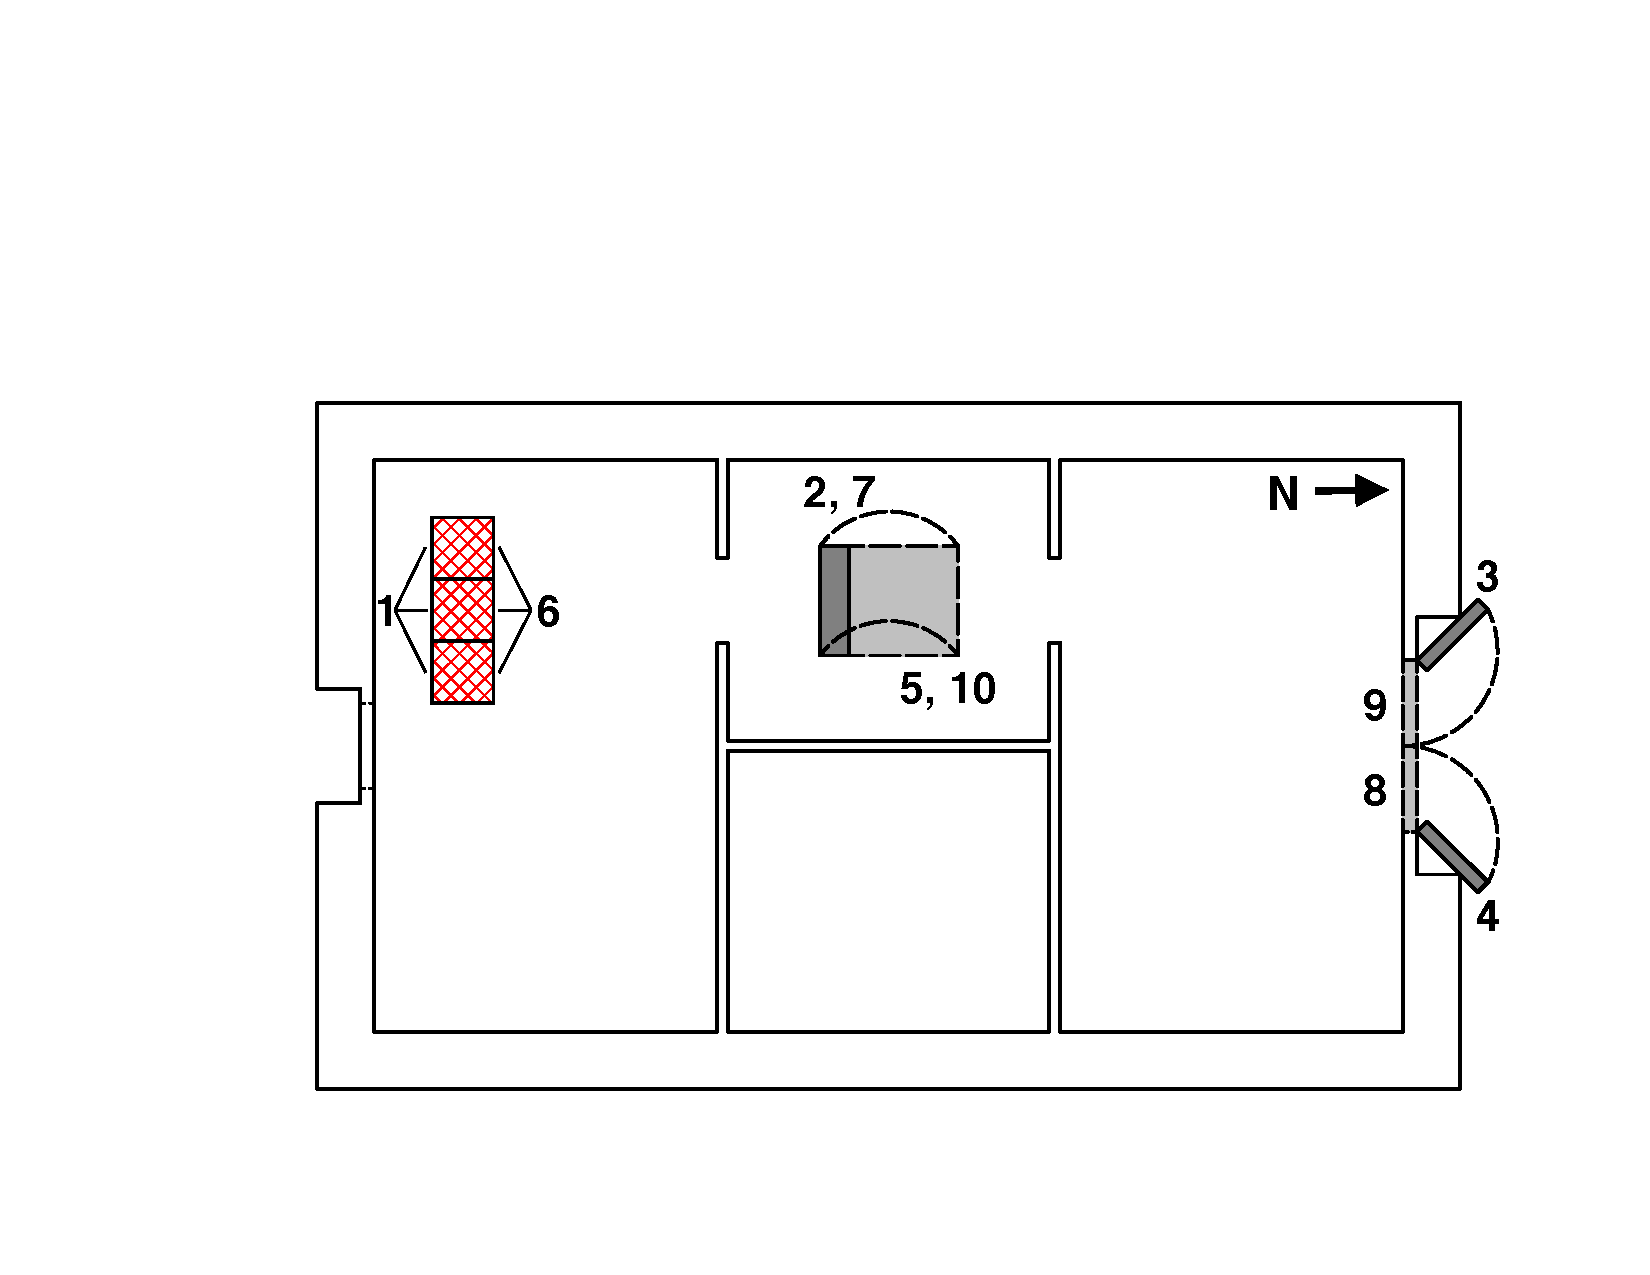
\includegraphics[width=0.76\columnwidth]{Figures/Floor_Plans/East_Structure_Test_5}
\end{minipage}
\renewcommand{\baselinestretch}{1}
\caption{Test~5 layout and event times.}
\label{fig:east_test_5}
\end{figure}
\FloatBarrier

% \begin{figure}[!ht]
% \begin{minipage}[b]{0.8\columnwidth}
% 	\begin{flushleft}
% 	\begin{tabular}{lccc}
% 	\multicolumn{4}{c}{\normalsize Event Times (s) for Test~6 Data File} \\
% 	\toprule
% 	\multicolumn{1}{c}{\textbf{Event}} 	& \textbf{Seq. 1}	& \textbf{Seq. 2} 	& \textbf{Seq. 3} 	\\
% 	\midrule
% 	~(1)~ All burners on 				&	0				&	565				&	1075			\\
% 	~(2)~ West double door opened 		&	116				&   685				&	1195			\\
% 	~(3)~ Roof vent opened 		    	&	207				&	747 			& 	1287 			\\
% 	~(4)~ All burners off 				&	327				&   868				&	1387			\\
% 	~(5)~ East double door opened		&	369				&   911				&	1446			\\
% 	~(6)~ Roof vent closed 				&	494				&   1040			&	N/A				\\
% 	~(7)~ East double door closed		&	522 			&	1012			&	N/A 			\\
% 	~(8)~ West double door closed		&	538 			&	1025			&	N/A				\\
% 	\bottomrule
% 	\end{tabular}
% 	\end{flushleft}
% \end{minipage}
% \begin{minipage}[b]{0.86\columnwidth}
% 	\vspace{15pt}
% 	\centering
% 	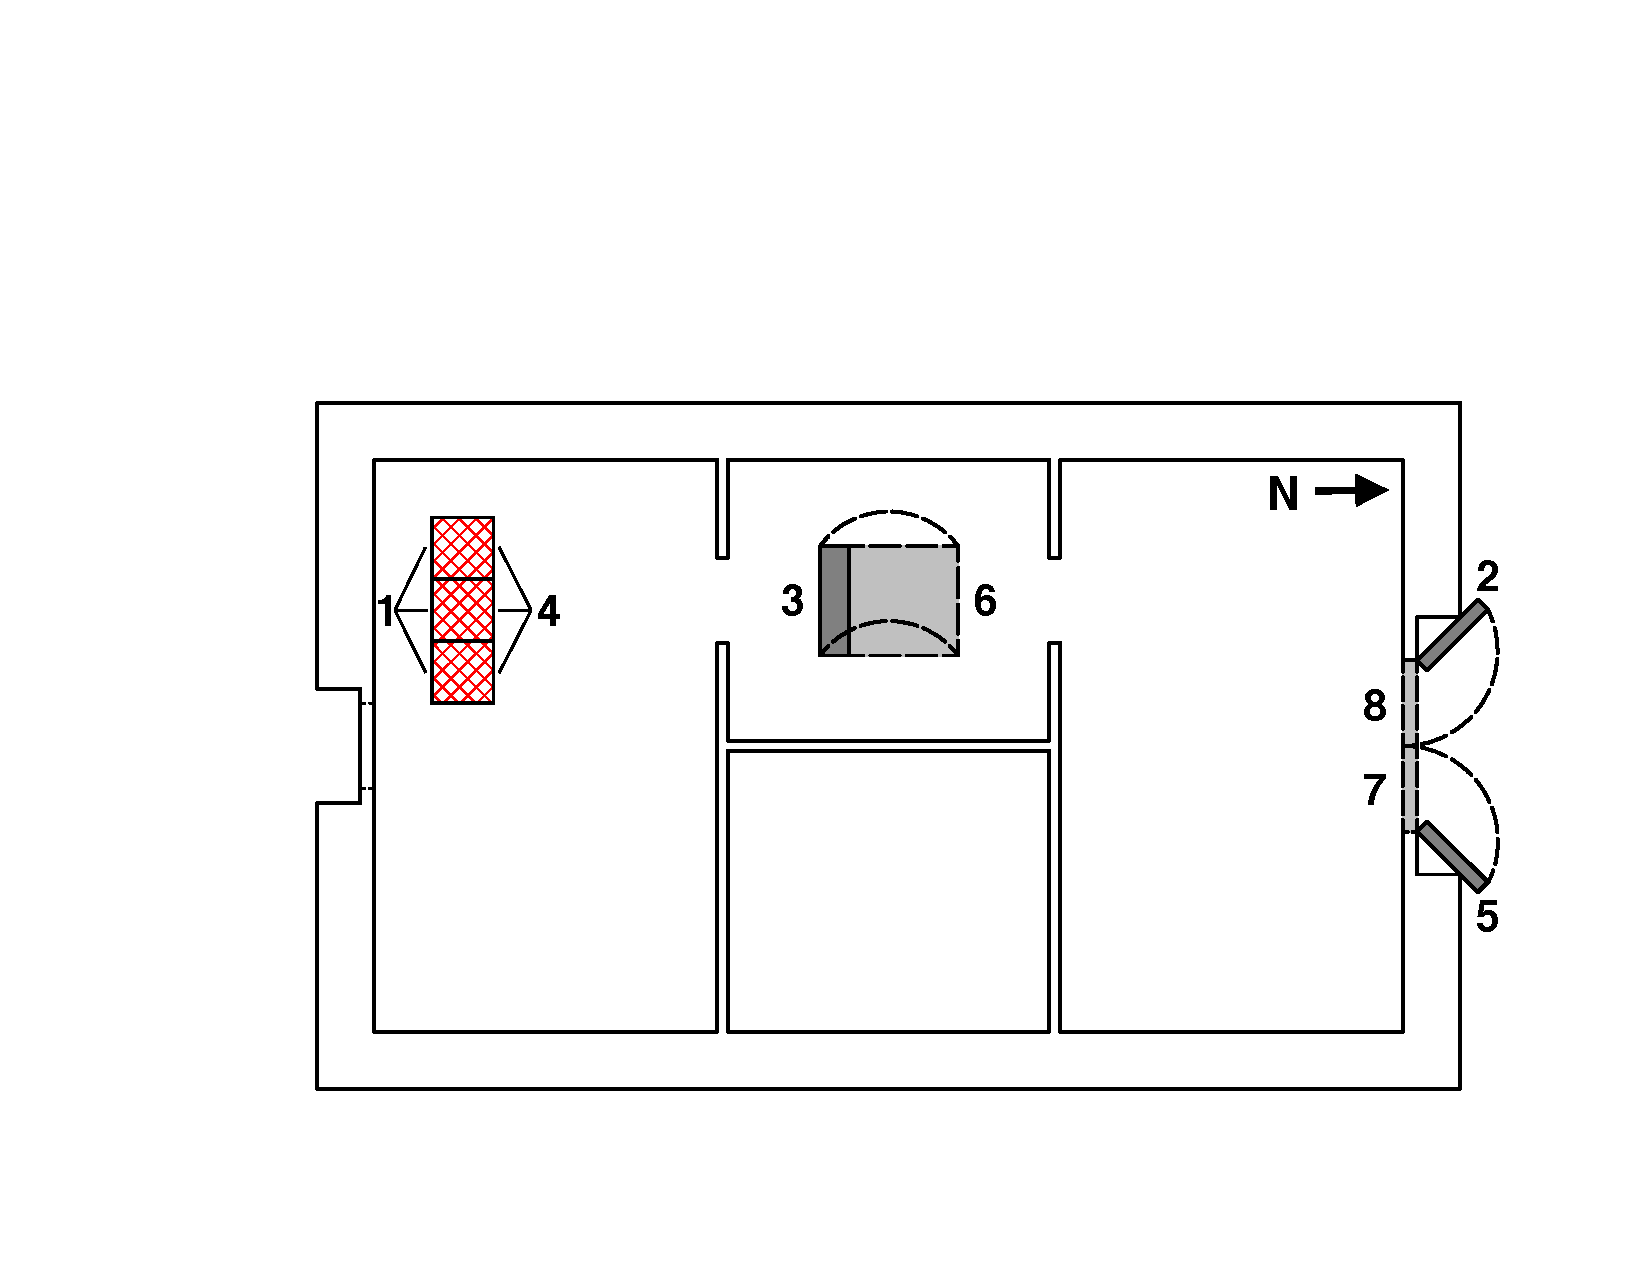
\includegraphics[width=\columnwidth]{Figures/Floor_Plans/East_Structure_Test_6}
% \end{minipage}
% \caption{Test~6 layout and event times.}
% \label{fig:east_test_6}
% \end{figure}
% \clearpage
% \renewcommand{\baselinestretch}{2}

\begin{figure}[!ht]
\renewcommand{\baselinestretch}{1}
\begin{minipage}[b]{0.98\columnwidth}
\begin{center}
	\begin{tabular}{lccc}
	\multicolumn{4}{c}{\normalsize Event Times (sec) for Test~6 Data File} \\
	\toprule
	\multicolumn{1}{c}{\textbf{Event}} 	& \textbf{Seq. 1}	& \textbf{Seq. 2} 	& \textbf{Seq. 3} 	\\
	\midrule
	~(1)~ All burners on 				&	0				&	565				&	1075			\\
	~(2)~ West double door opened 		&	116				&   685				&	1195			\\
	~(3)~ Roof vent opened 		    	&	207				&	747 			& 	1287 			\\
	~(4)~ All burners off 				&	327				&   868				&	1387			\\
	~(5)~ East double door opened		&	369				&   911				&	1446			\\
	~(6)~ Roof vent closed 				&	494				&   1040			&	N/A				\\
	~(7)~ East double door closed		&	522 			&	1012			&	N/A 			\\
	~(8)~ West double door closed		&	538 			&	1025			&	N/A				\\
	\bottomrule
	\end{tabular}
	% \begin{tabular}{|l|c|c|c|}
	% \multicolumn{4}{c}{Event Times (sec) for Test~6 Data File}
	% \vspace{5pt} \\
	% \hline
	% \multicolumn{1}{|c|}{Event}		    & Seq. 1 		  	& Seq. 2 			& 	Seq. 3 			\\
	% \hline \hline
	% ~(1)~ All burners on 				&	0				&	565				&	1075			\\
	% ~(2)~ West double door opened 		&	116				&   685				&	1195			\\
	% ~(3)~ Roof vent opened 		    	&	207				&	747 			& 	1287 			\\
	% ~(4)~ All burners off 				&	327				&   868				&	1387			\\
	% ~(5)~ East double door opened		&	369				&   911				&	1446			\\
	% ~(6)~ Roof vent closed 				&	494				&   1040			&	N/A				\\
	% ~(7)~ East double door closed		&	522 			&	1012			&	N/A 			\\
	% ~(8)~ West double door closed		&	538 			&	1025			&	N/A				\\
	% \hline
	% \end{tabular}
\end{center}
\end{minipage}
\begin{minipage}[b]{\columnwidth}
	\vspace{20pt}
	\centering
	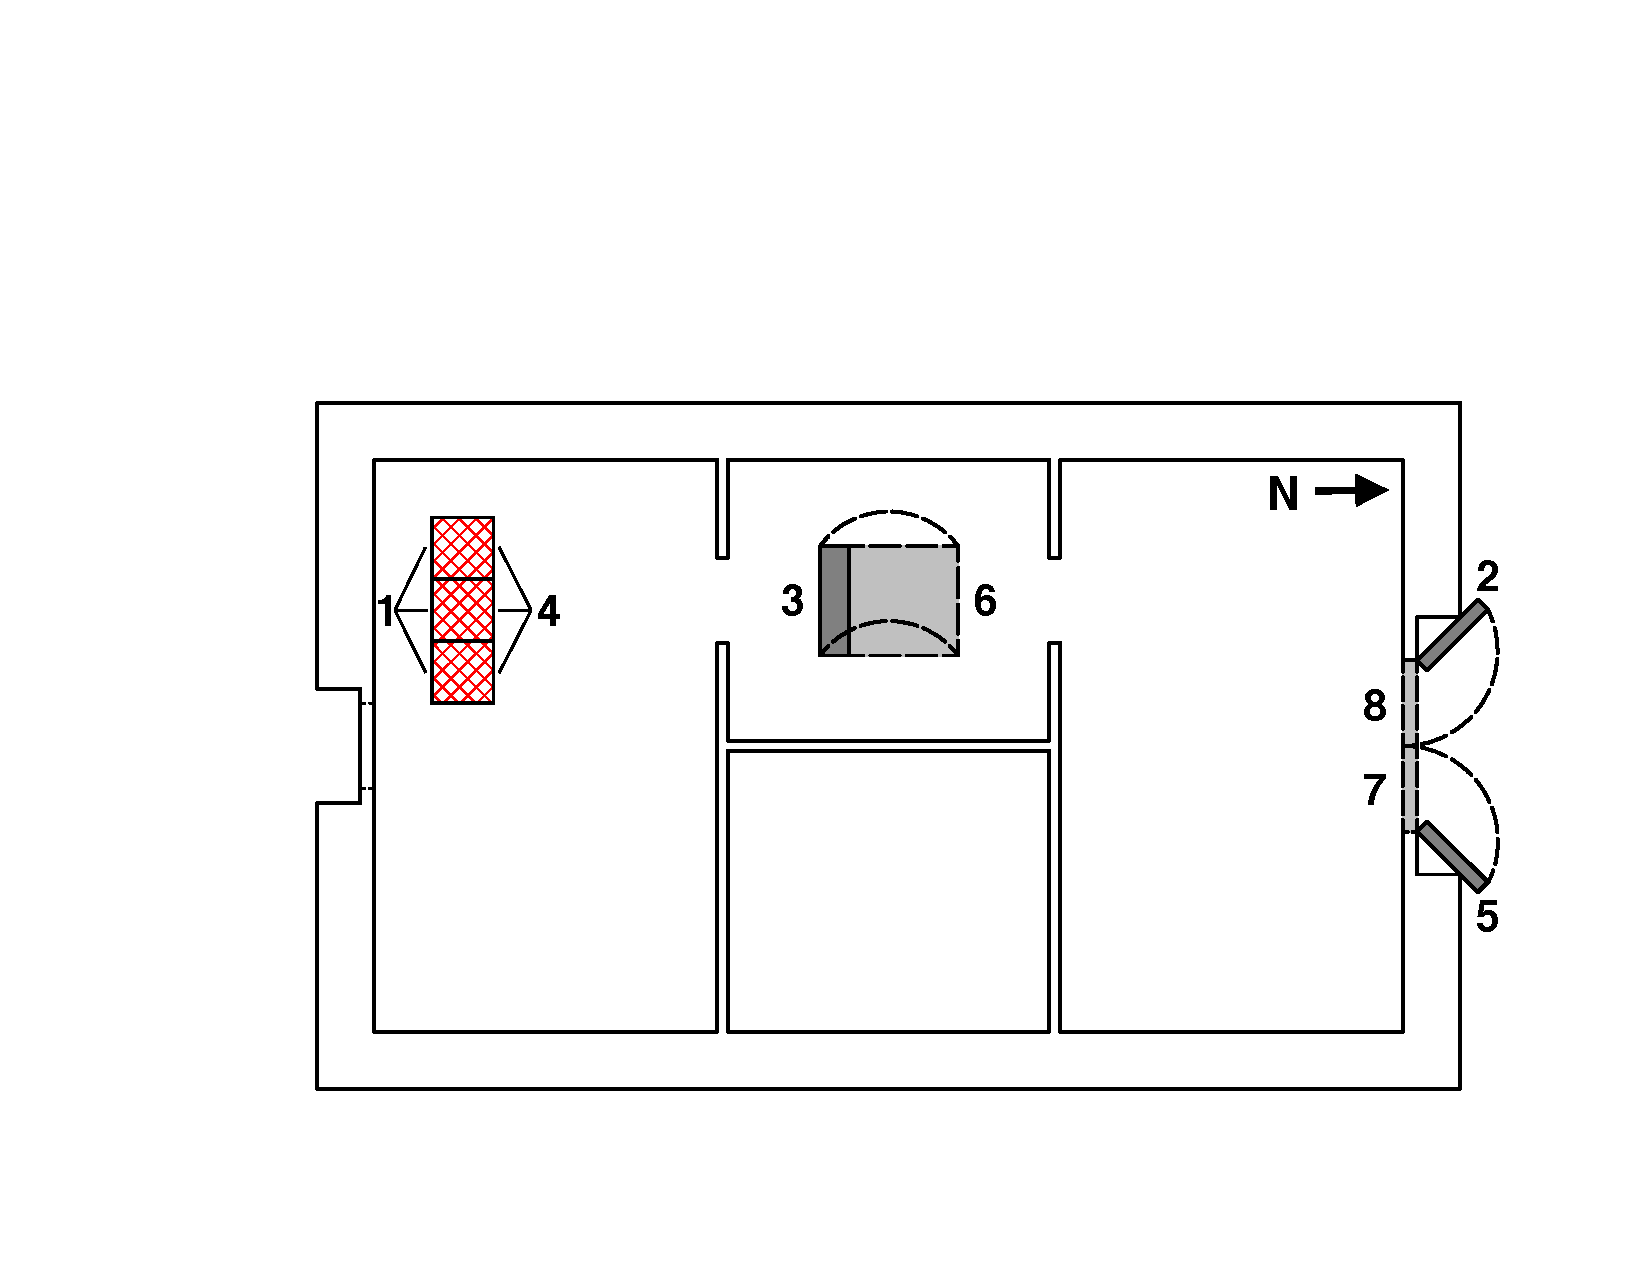
\includegraphics[width=0.8\columnwidth]{Figures/Floor_Plans/East_Structure_Test_6}
\end{minipage}
\renewcommand{\baselinestretch}{1}
\caption{Test~6 layout and event times.}
\label{fig:east_test_6}
\end{figure}
\FloatBarrier

\section{West Structure Tests}

Four of the gas burner experiments, Tests~22--25, were conducted in the West Structure. Table~\ref{table:HRR_Tests_22-25} lists the calculated heat release rate for each test. Similar to Tests~5 and 6, Tests~22--25 had a duration on the order of seconds between the ignition of each burner, so only the heat release rate for all three burners is reported.

\renewcommand{\baselinestretch}{1}
% \begin{table}[h]
% \caption[Heat Release Rates for Tests~22--25.]{Heat Release Rates (kW) for Tests~22--25.}
% \begin{center}
% \begin{tabular}{|c|c|}
% \hline
%  % & \textbf{Heat Release Rate (kW)} \\
% \multirow{2}{*}{Test~\#}    & Heat Release Rate for \\ 
% 							& All Burners Ignited (kW) \\
% \hline \hline
% 22				&     	1240 	  \\
% 23				&     	1290 	  \\
% 24				& 	    1270 	  \\
% 25				&     	1270 	  \\
% \hline
% \end{tabular}
% \end{center}
% \label{table:HRR_Tests_22-25}
% \end{table}
% \renewcommand{\baselinestretch}{2}
\begin{table}[!ht]
\caption{Heat Release Rates for Tests~22--25.}
\begin{center}
\begin{tabular}{lc}
 \toprule
					& 	\textbf{Heat Release Rate (kW)}	\\
\textbf{Test}		& 	\textbf{All Burners On} \\
 \midrule
Test 22				&     	1240 	  \\
Test 23				&     	1290 	  \\
Test 24				& 	    1270 	  \\
Test 25				&     	1270 	  \\
\bottomrule
\end{tabular}
\end{center}
\label{table:HRR_Tests_22-25}
\end{table}
% \renewcommand{\baselinestretch}{2}
\FloatBarrier
\subsection{Tests~22 \& 23}

Tests~22 and 23 followed nearly identical procedures. The starting configuration for Test~22 had the second-story, south exterior door in the opened position, while the starting configuration for Test~23 had the same door in the closed position. Figure~\ref{fig:west_test_22} includes a floor plan schematic and table of event times corresponding to the data files for Tests~22 and 23. A 0.61~m (2.0~ft) diameter PPV fan located 2.3~m (7.5~ft) away from the first level double doors and aimed at the center of the two doors was used towards the end of both tests.
% \begin{figure}[!ht]
% \begin{minipage}[b]{0.8\columnwidth}
% 	\begin{flushleft}
% 	\begin{tabular}{lcc}
% 	\multicolumn{3}{c}{Event Times (s) for Tests~22--23 Data Files} \\
% 	\toprule
% 	\multicolumn{1}{c}{\textbf{Event}} 			& \textbf{Test 22}	& \textbf{Test 23} \\
% 	\midrule
% 	~(1)~  All burners on 						&   0	  			&	 0			\\
% 	~(2)~  2nd floor west double door opened 	&   194		  		&    130		\\
% 	~(3)~  1st floor west double door opened 	&	314		  		&    252 	 	\\
% 	~(4)~  1st floor east double door opened 	&   450			  	&    371		\\
% 	~(5)~  2nd floor south exterior door closed &   511		  		&    N/A		\\
% 	~(6)~  2nd floor east double door opened	&   585			  	&    498		\\
% 	~(7)~  PPV fan on 							&   652			  	&    612		\\
% 	~(8)~  PPV fan off              			&   798			  	&    761		\\
% 	~(9)~  All burners off 						&   829			  	&    794		\\
% 	(10)   2nd floor south exterior door opened &   899			  	&    849		\\
% 	(11)   PPV fan on 	 						&   1065		  	&    940		\\
% 	(12)   2nd floor south exterior door closed &   1176		  	&    N/A		\\
% 	\bottomrule
% 	\end{tabular}
% 	\end{flushleft}
% \end{minipage}
% \begin{minipage}[b]{0.9\columnwidth}
% 	\vspace{15pt}
% 	\centering
% 	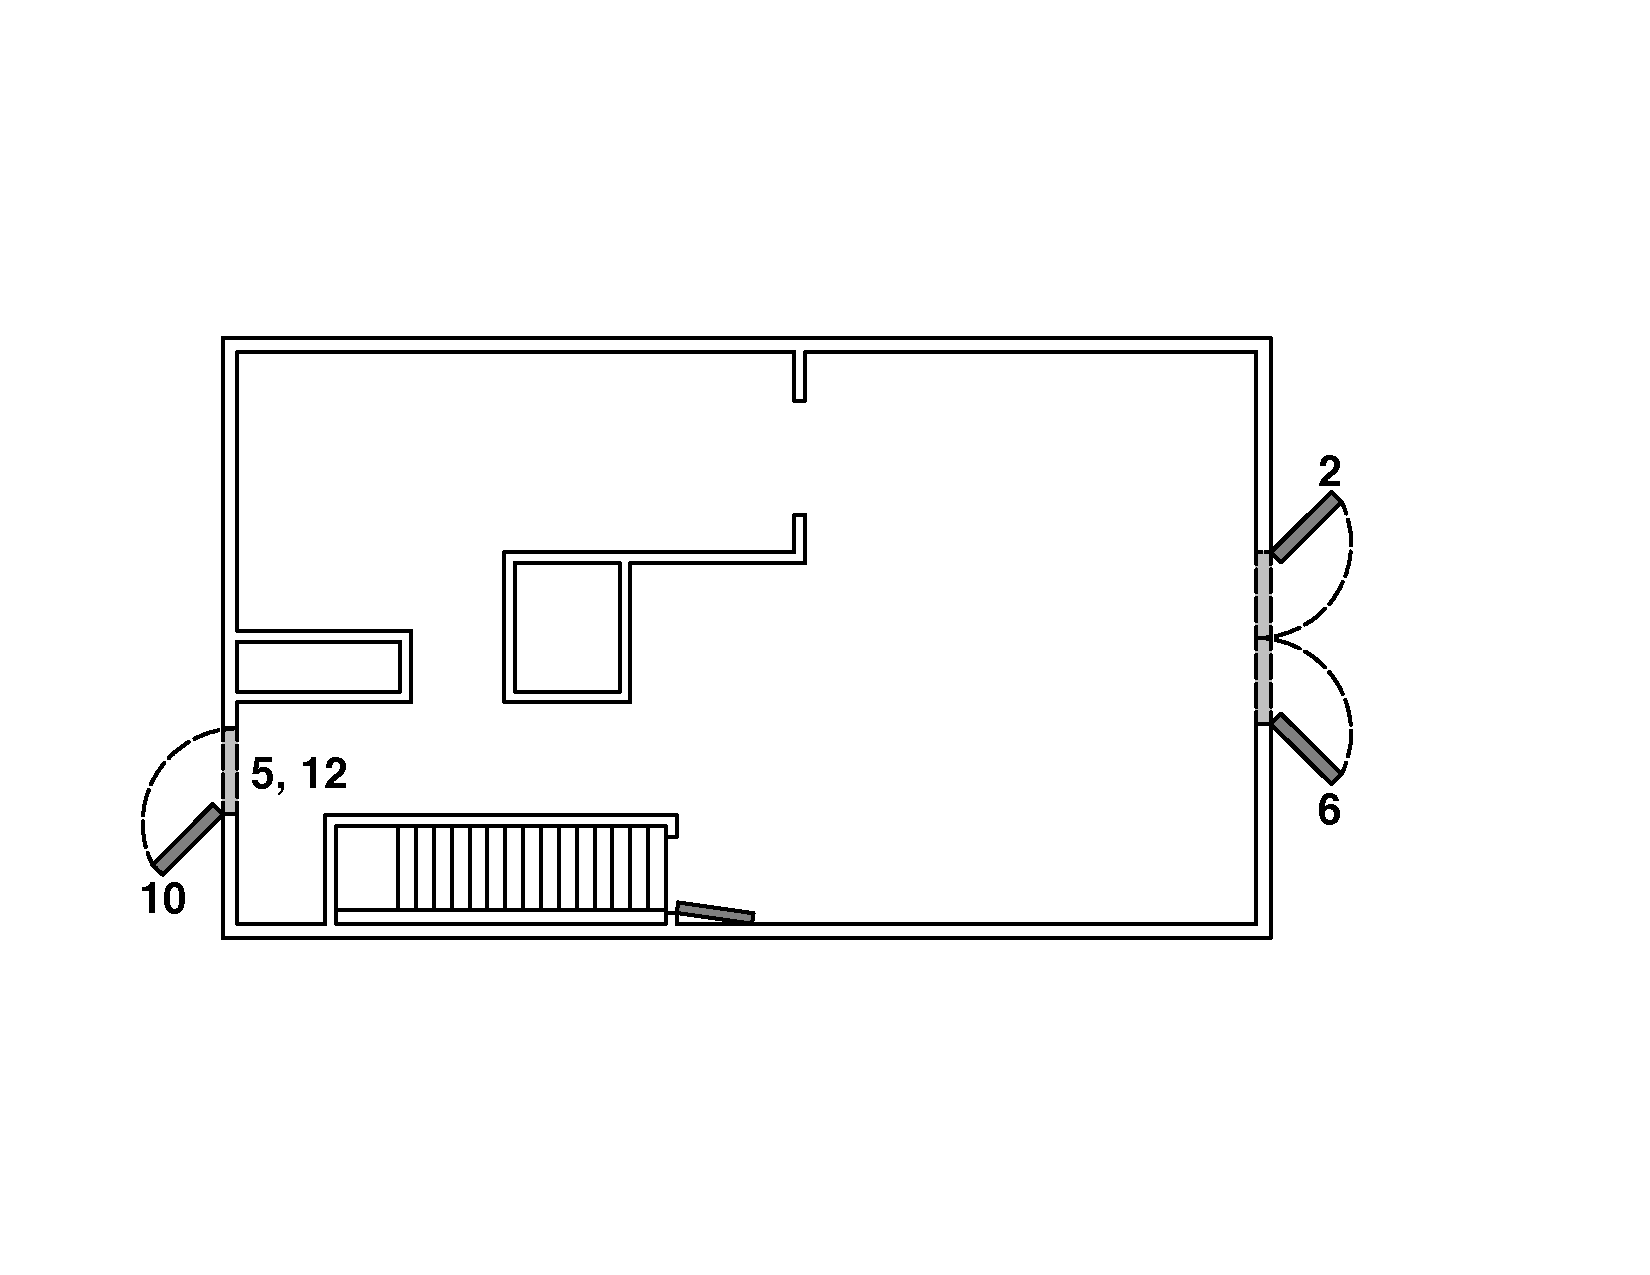
\includegraphics[width=\columnwidth]{Figures/Floor_Plans/West_Structure_2nd_Floor_Test_22}
% 	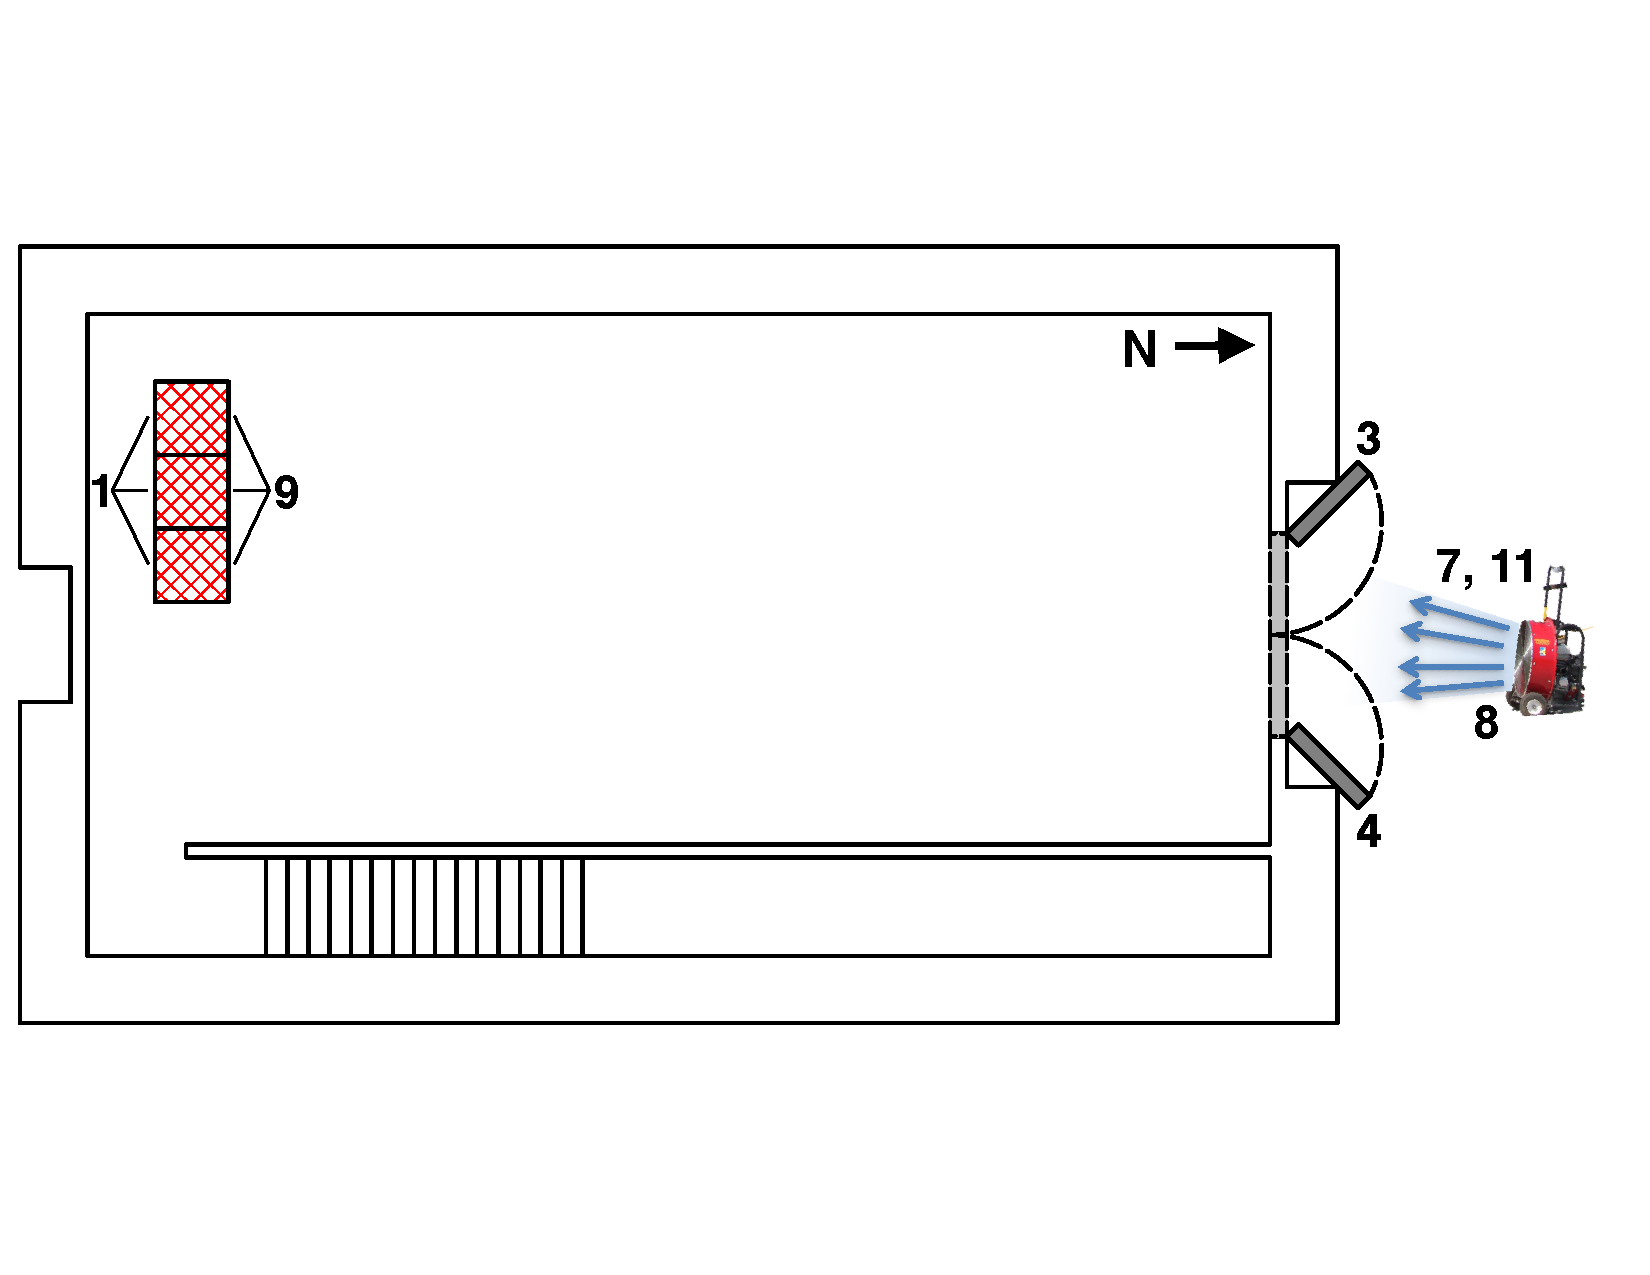
\includegraphics[width=0.95\columnwidth]{Figures/Floor_Plans/West_Structure_1st_Floor_Test_22}
% \end{minipage}
% \caption{Tests 22--23 layout and event times.}
% \label{fig:west_test_22}
% \end{figure}

\begin{figure}[!ht]
\renewcommand{\baselinestretch}{1}
\begin{minipage}[b]{0.88\columnwidth}
\begin{center}
	\begin{tabular}{lcc}
	\multicolumn{3}{c}{Event Times (sec) for Tests~22--23 Data Files} \\
	\toprule
	\multicolumn{1}{c}{\textbf{Event}} 			& \textbf{Test 22}	& \textbf{Test 23} \\
	\midrule
	~(1)~  All burners on 						&   0	  			&	 0			\\
	~(2)~  2nd floor west double door opened 	&   194		  		&    130		\\
	~(3)~  1st floor west double door opened 	&	314		  		&    252 	 	\\
	~(4)~  1st floor east double door opened 	&   450			  	&    371		\\
	~(5)~  2nd floor south exterior door closed &   511		  		&    N/A		\\
	~(6)~  2nd floor east double door opened	&   585			  	&    498		\\
	~(7)~  PPV fan on 							&   652			  	&    612		\\
	~(8)~  PPV fan off              			&   798			  	&    761		\\
	~(9)~  All burners off 						&   829			  	&    794		\\
	(10)   2nd floor south exterior door opened &   899			  	&    849		\\
	(11)   PPV fan on 	 						&   1065		  	&    940		\\
	(12)   2nd floor south exterior door closed &   1176		  	&    N/A		\\
	\bottomrule
	\end{tabular}
	% \begin{tabular}{|l|c|c|}
	% \multicolumn{3}{c}{Event Times (sec) for Tests~22--23 Data Files}
	% \vspace{5pt} \\
	% \hline
	% \multicolumn{1}{|c|}{Event}		    		& Test 22		  	& Test 23		\\
	% \hline \hline
	% ~(1)~  All burners on 						&   0	  			&	 0			\\
	% ~(2)~  2nd floor west double door opened 	&   194		  		&    130		\\
	% ~(3)~  1st floor west double door opened 	&	314		  		&    252 	 	\\
	% ~(4)~  1st floor east double door opened 	&   450			  	&    371		\\
	% ~(5)~  2nd floor south exterior door closed &   511		  		&    N/A		\\
	% ~(6)~  2nd floor east double door opened	&   585			  	&    498		\\
	% ~(7)~  PPV fan on 							&   652			  	&    612		\\
	% ~(8)~  PPV fan off              			&   798			  	&    761		\\
	% ~(9)~  All burners off 						&   829			  	&    794		\\
	% (10)   2nd floor south exterior door opened &   899			  	&    849		\\
	% (11)   PPV fan on 	 						&   1065		  	&    940		\\
	% (12)   2nd floor south exterior door closed &   1176		  	&    N/A		\\
	% \hline
	% \end{tabular}
\end{center}
\end{minipage}
\begin{minipage}[b]{\columnwidth}
	\vspace{15pt}
	\centering
	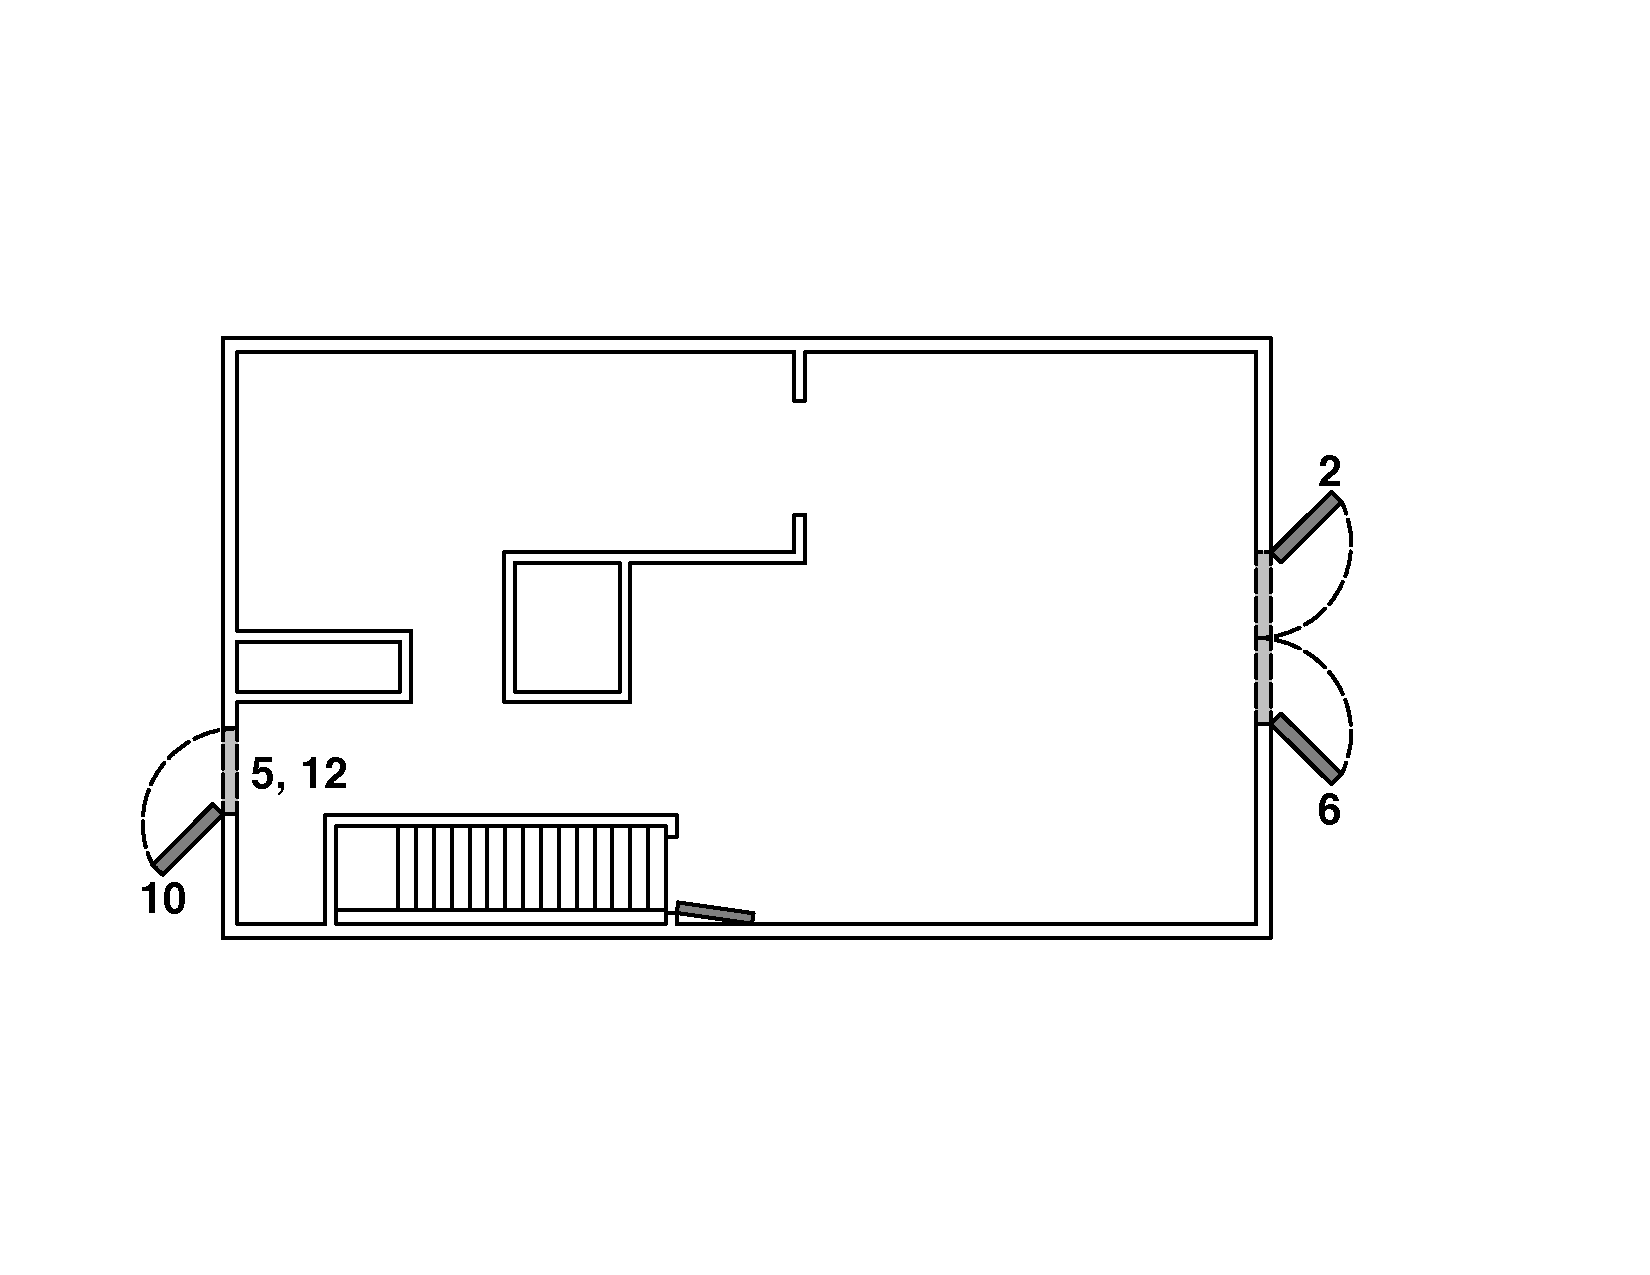
\includegraphics[width=\columnwidth]{Figures/Floor_Plans/West_Structure_2nd_Floor_Test_22}
	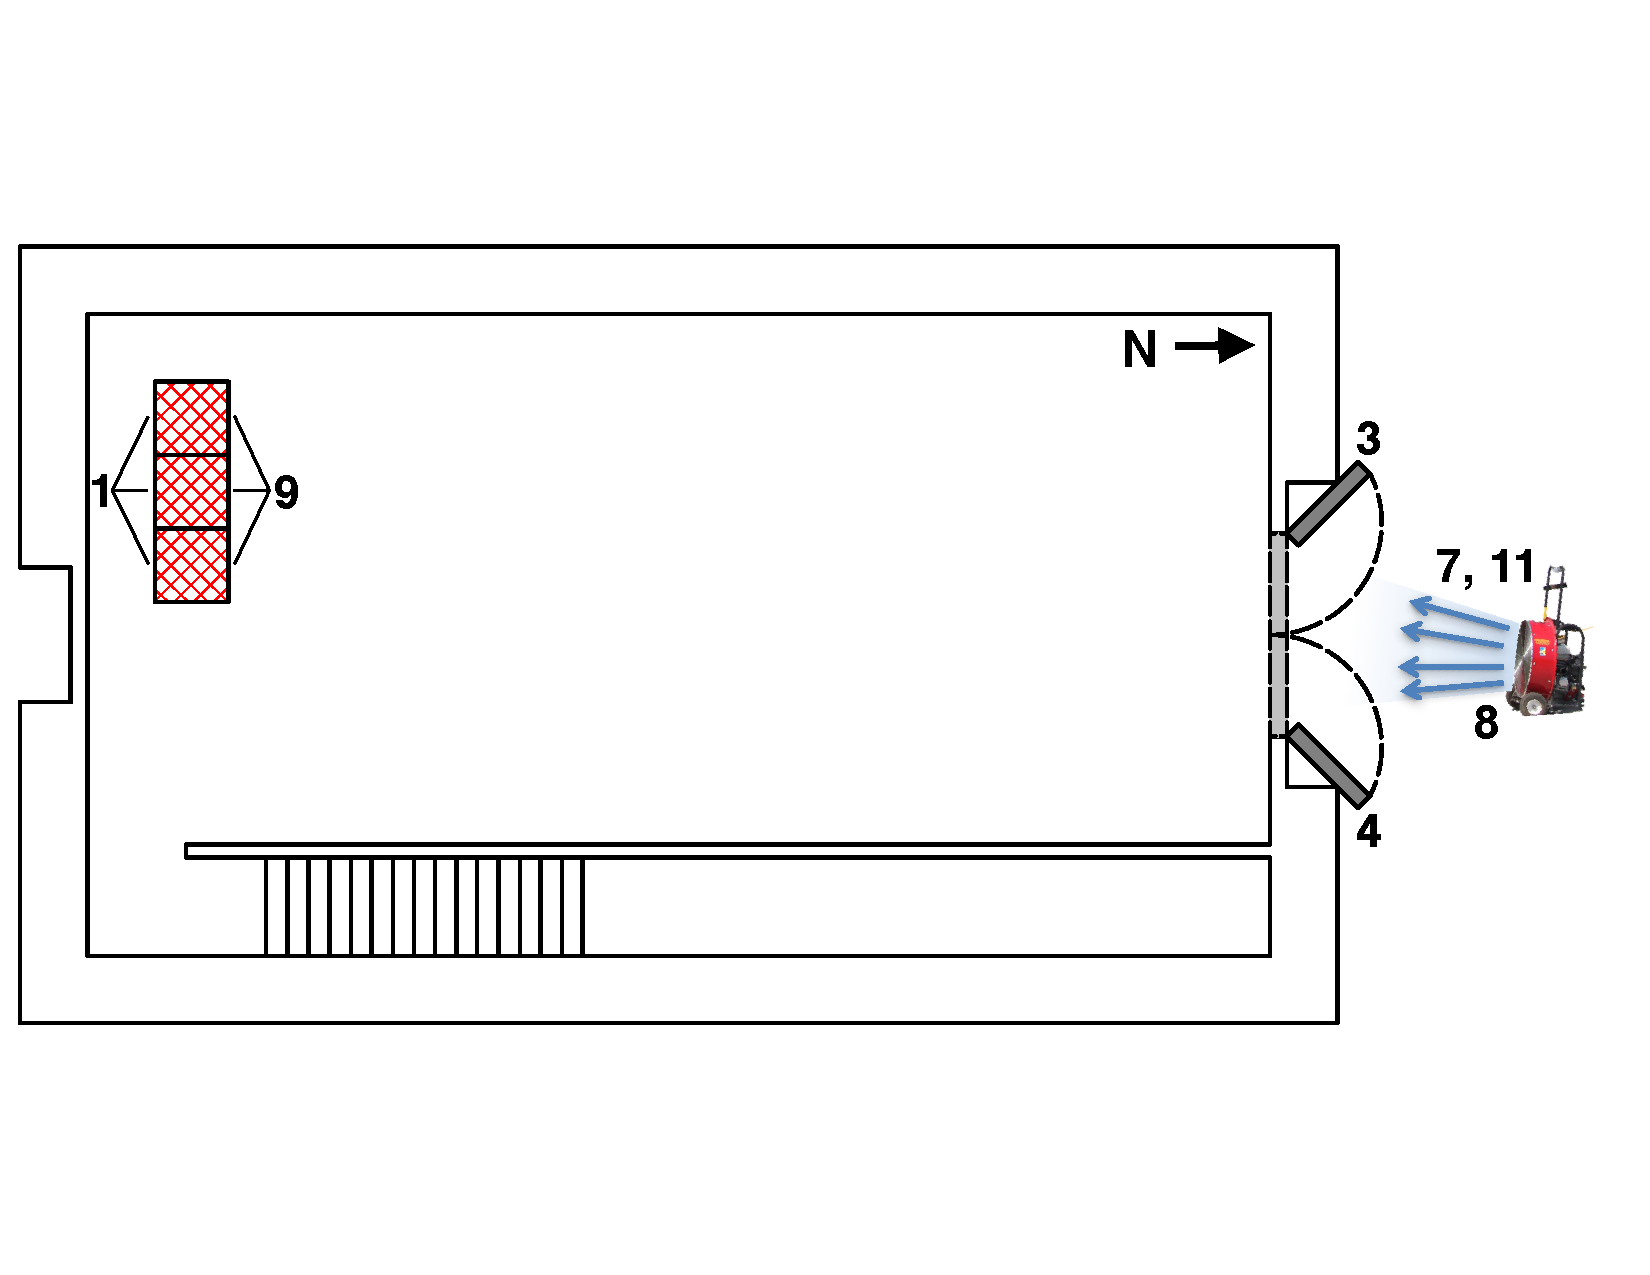
\includegraphics[width=0.95\columnwidth]{Figures/Floor_Plans/West_Structure_1st_Floor_Test_22}
\end{minipage}
\renewcommand{\baselinestretch}{1}
\caption{Tests 22--23 layout and event times.}
\label{fig:west_test_22}
\end{figure}
\FloatBarrier

\subsection{Tests~24 \& 25}

As with Tests~22 and 23, Tests~24 and 25 followed a nearly identical procedure. The starting configuration for Test~24 had the south exterior door on the second level in the opened position, while the starting configuration for Test~25 had the same door in the closed position. During both tests, the stairwell door was unable to completely close. When it was in the ``closed'' position at the beginning of each test, there was a 152~mm (6.0~in) gap between the door and its frame. Figure~\ref{fig:west_test_24} includes a floor plan schematic and table of event times corresponding to the data files for Tests~24 and 25. A 0.61~m (2.0~ft) diameter PPV fan located 2.3~m (7.5~ft) away from the first level double doors and aimed at the center of the west double door was used towards the end of both tests.

% \begin{figure}[!ht]
% \begin{minipage}[b]{0.8\columnwidth}
% 	\begin{flushleft}
% 	\begin{tabular}{lcc}
% 	\multicolumn{3}{c}{Event Times (s) for Tests 24--25 Data Files} \\
% 	\toprule
% 	\multicolumn{1}{c}{\textbf{Event}} 			& \textbf{Test 24}	& \textbf{Test 25} \\
% 	\midrule
% 	~(1)~ All burners on 						&   0		  		&	 0			\\
% 	~(2)~ Interior stairwell door opened 		&   144		  		&    112		\\
% 	~(3)~ 1st floor west double door opened 	&	265		  		&    244 	 	\\
% 	~(4)~ 2nd floor west double door opened 	&   383			  	&    353		\\
% 	~(5)~ 2nd floor south exterior door closed	&   452			  	&    N/A		\\
% 	~(6)~ 2nd floor south exterior door opened	&   502			  	&    474		\\
% 	~(7)~ PPV fan on 							&   624			  	&    594 		\\
% 	~(8)~ All burners off 						&   746 		  	&    721		\\
% 	~(9)~ 2nd floor east double door opened 	&   877			  	&    N/A		\\
% 	(10)  1st floor east double door opened		& 	N/A 			& 	 836		\\
% 	\bottomrule
% 	\end{tabular}
% 	\end{flushleft}
% \end{minipage}
% \begin{minipage}[b]{0.9\columnwidth}
% 	\vspace{15pt}
% 	\centering
% 	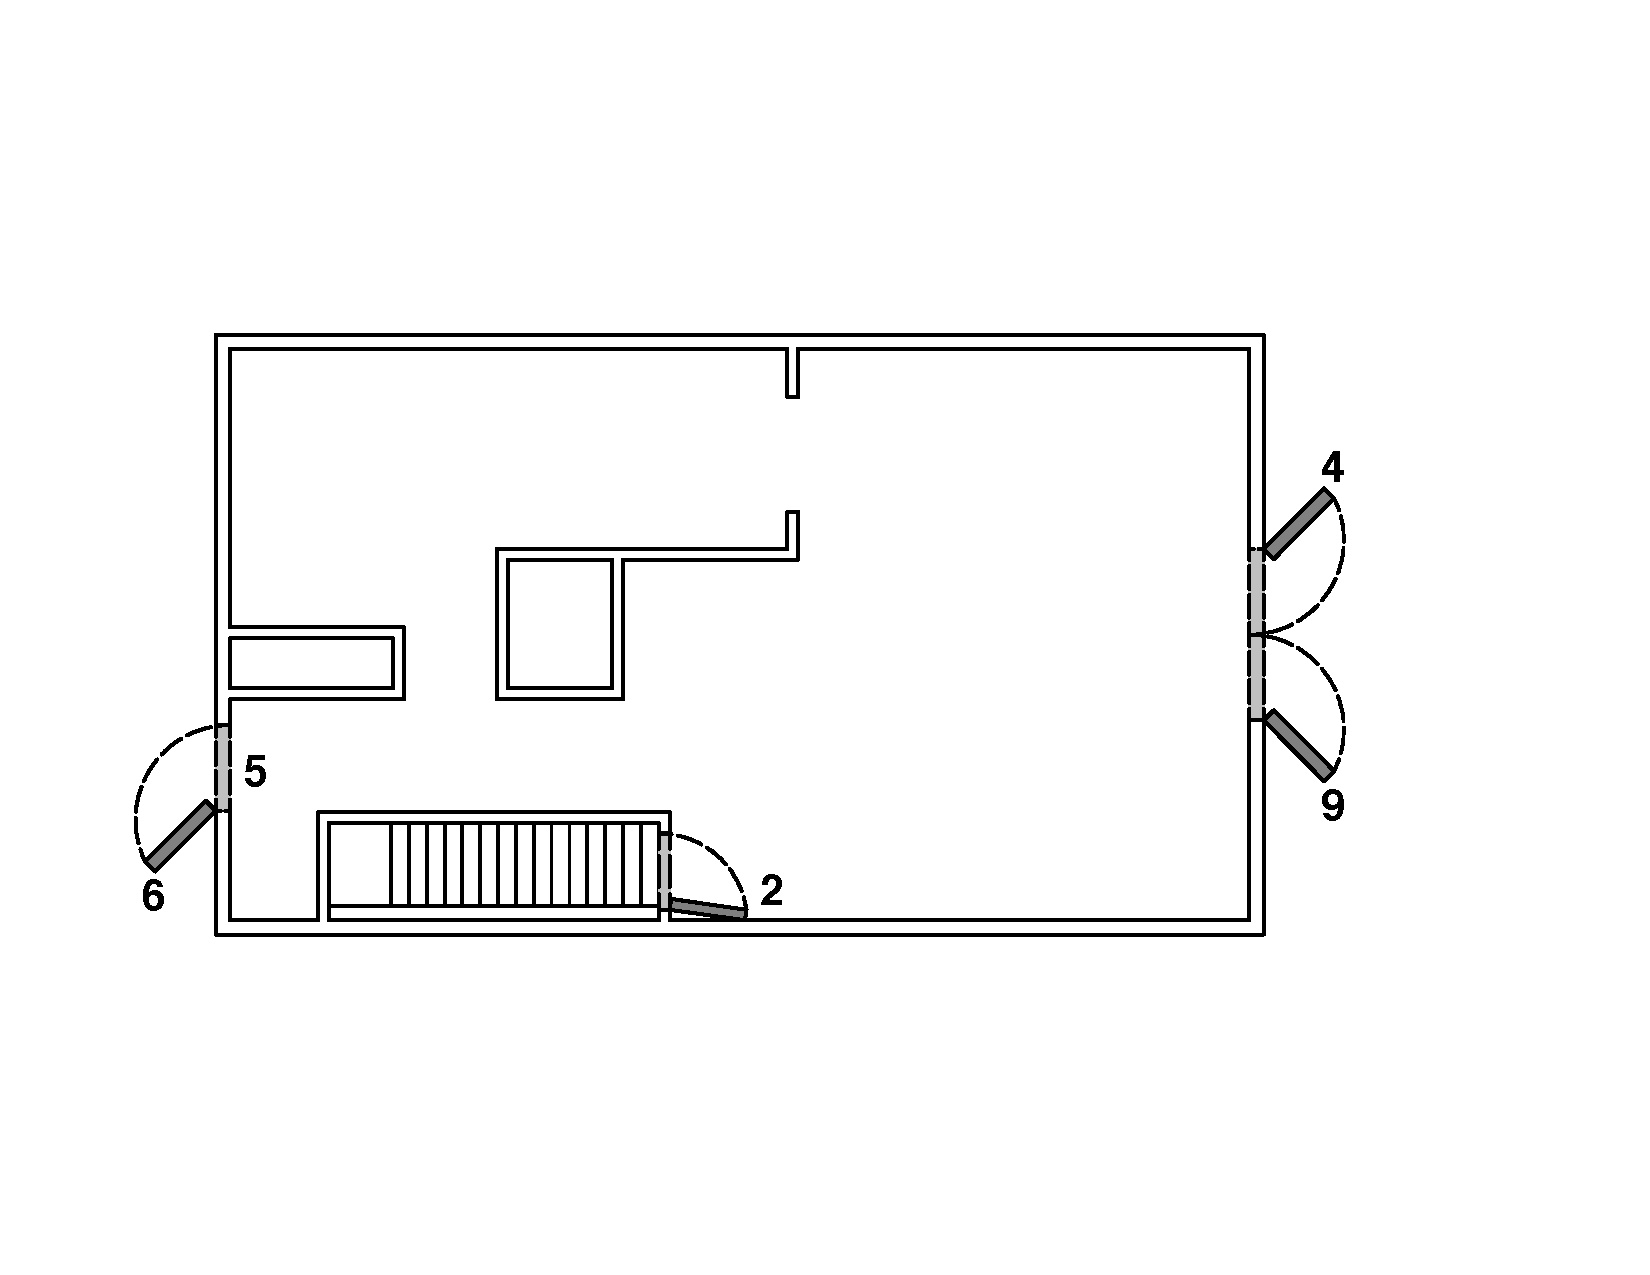
\includegraphics[width=\columnwidth]{Figures/Floor_Plans/West_Structure_2nd_Floor_Test_24}
% 	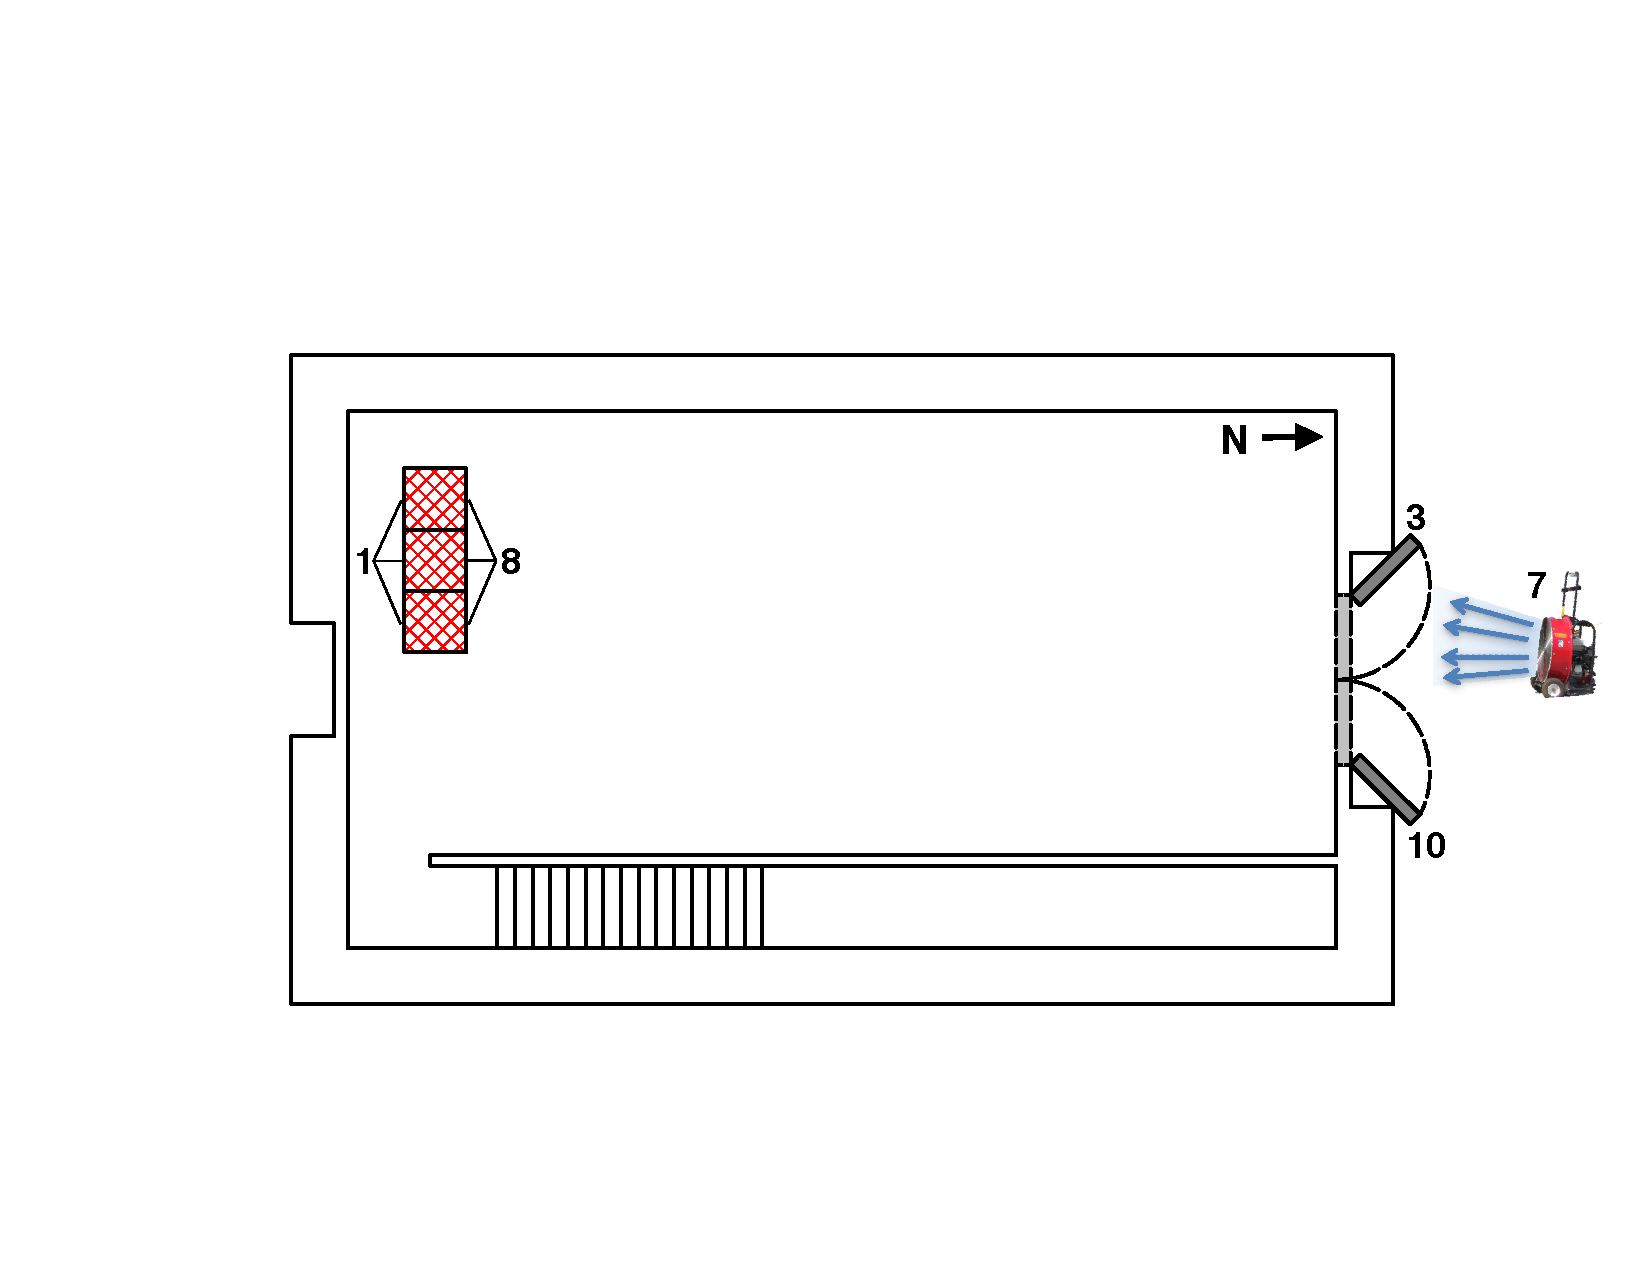
\includegraphics[width=0.95\columnwidth]{Figures/Floor_Plans/West_Structure_1st_Floor_Test_24}
% \end{minipage}
% \caption{Tests 24--25 layout and event times.}
% \label{fig:west_test_24}
% \end{figure}
% \clearpage

\begin{figure}[!ht]
\renewcommand{\baselinestretch}{1}
\begin{minipage}[b]{0.88\columnwidth}
\begin{center}
	% \begin{tabular}{|l|c|c|}
	% \multicolumn{3}{c}{Event Times (sec) for Tests~24--25 Data Files}
	% \vspace{5pt} \\
	% \hline
	% \multicolumn{1}{|c|}{Event}		    		& Test 24		  	& Test 25		\\
	% \hline \hline
	% ~(1)~ All burners on 						&   0		  		&	 0			\\
	% ~(2)~ Interior stairwell door opened 		&   144		  		&    112		\\
	% ~(3)~ 1st floor west double door opened 	&	265		  		&    244 	 	\\
	% ~(4)~ 2nd floor west double door opened 	&   383			  	&    353		\\
	% ~(5)~ 2nd floor south exterior door closed	&   452			  	&    N/A		\\
	% ~(6)~ 2nd floor south exterior door opened	&   502			  	&    474		\\
	% ~(7)~ PPV fan on 							&   624			  	&    594 		\\
	% ~(8)~ All burners off 						&   746 		  	&    721		\\
	% ~(9)~ 2nd floor east double door opened 	&   877			  	&    N/A		\\
	% (10)  1st floor east double door opened		& 	N/A 			& 	 836		\\
	% \hline
	% \end{tabular}
	\begin{tabular}{lcc}
	\multicolumn{3}{c}{Event Times (sec) for Tests 24--25 Data Files} \\
	\toprule
	\multicolumn{1}{c}{\textbf{Event}} 			& \textbf{Test 24}	& \textbf{Test 25} \\
	\midrule
	~(1)~ All burners on 						&   0		  		&	 0			\\
	~(2)~ Interior stairwell door opened 		&   144		  		&    112		\\
	~(3)~ 1st floor west double door opened 	&	265		  		&    244 	 	\\
	~(4)~ 2nd floor west double door opened 	&   383			  	&    353		\\
	~(5)~ 2nd floor south exterior door closed	&   452			  	&    N/A		\\
	~(6)~ 2nd floor south exterior door opened	&   502			  	&    474		\\
	~(7)~ PPV fan on 							&   624			  	&    594 		\\
	~(8)~ All burners off 						&   746 		  	&    721		\\
	~(9)~ 2nd floor east double door opened 	&   877			  	&    N/A		\\
	(10)  1st floor east double door opened		& 	N/A 			& 	 836		\\
	\bottomrule
	\end{tabular}
\end{center}
\end{minipage}
\begin{minipage}[b]{\columnwidth}
	\vspace{15pt}
	\centering
	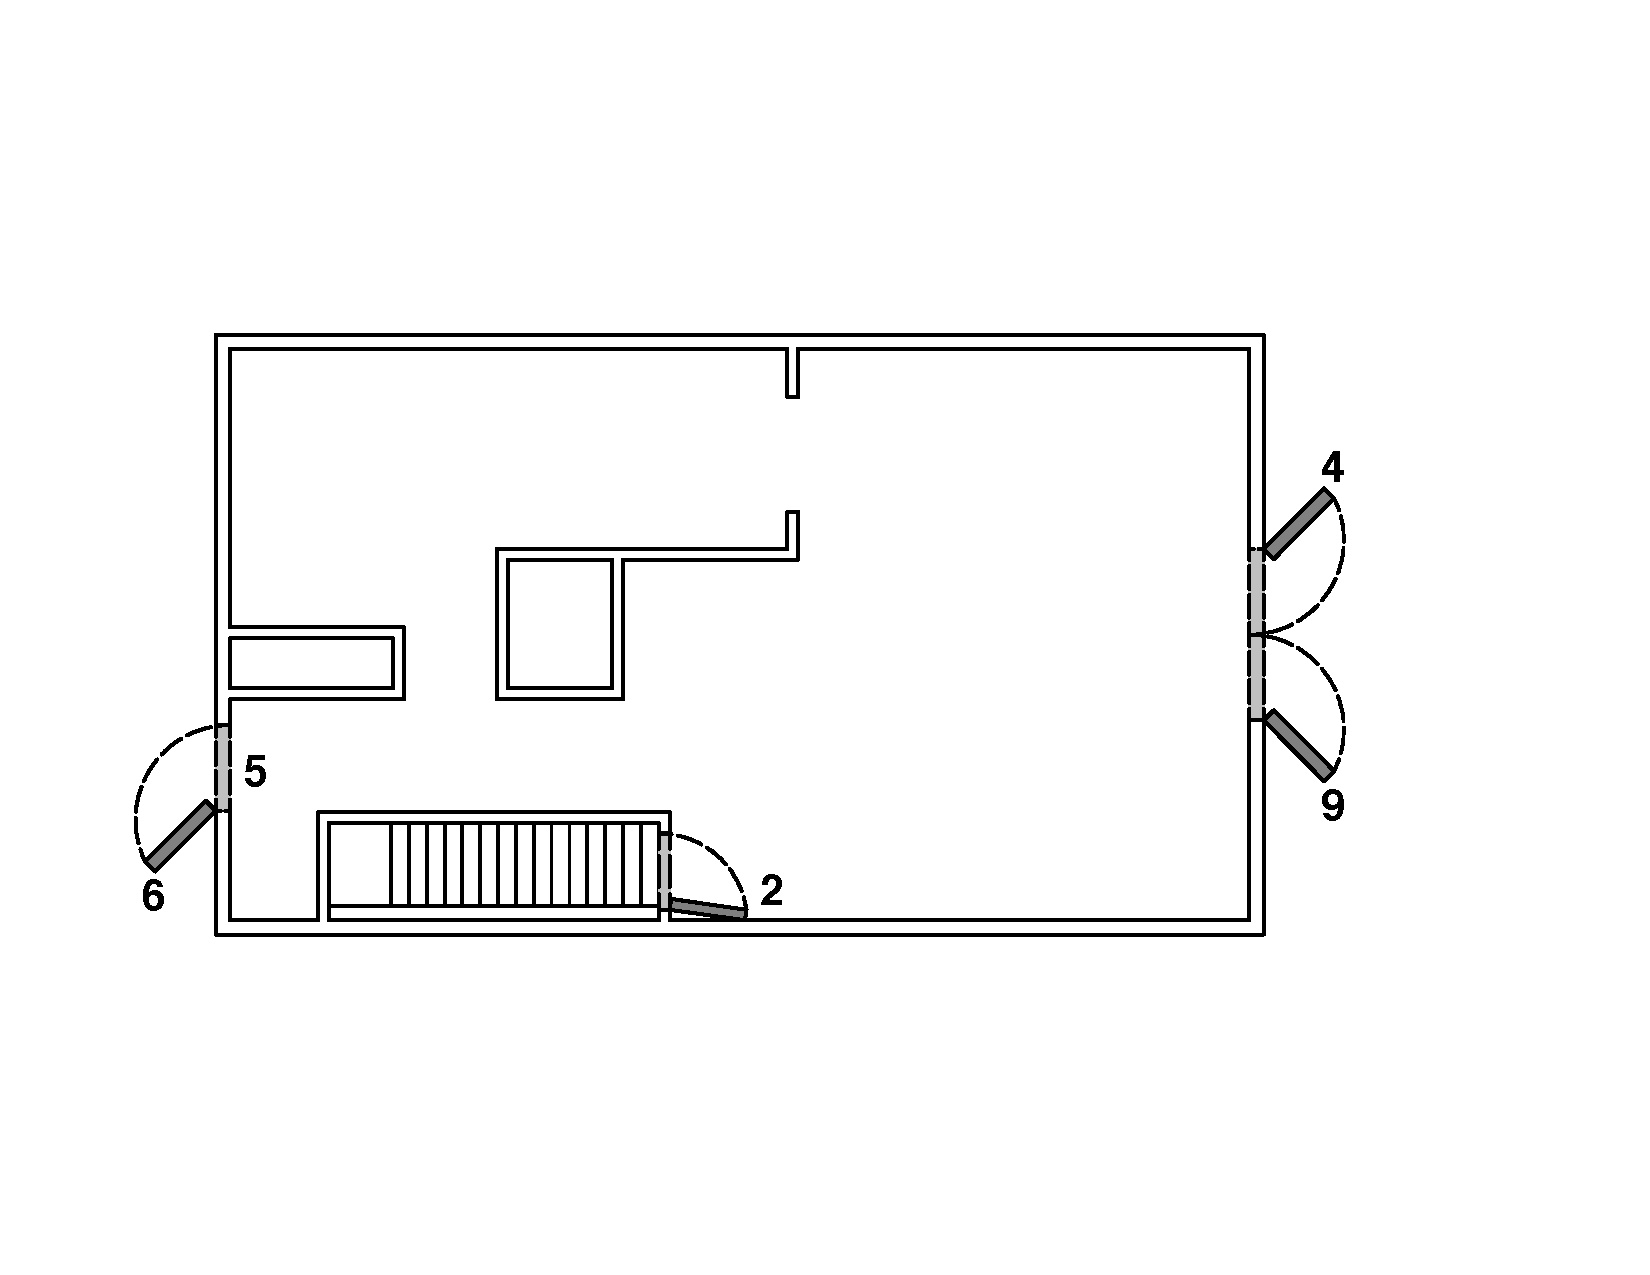
\includegraphics[width=\columnwidth]{Figures/Floor_Plans/West_Structure_2nd_Floor_Test_24}
	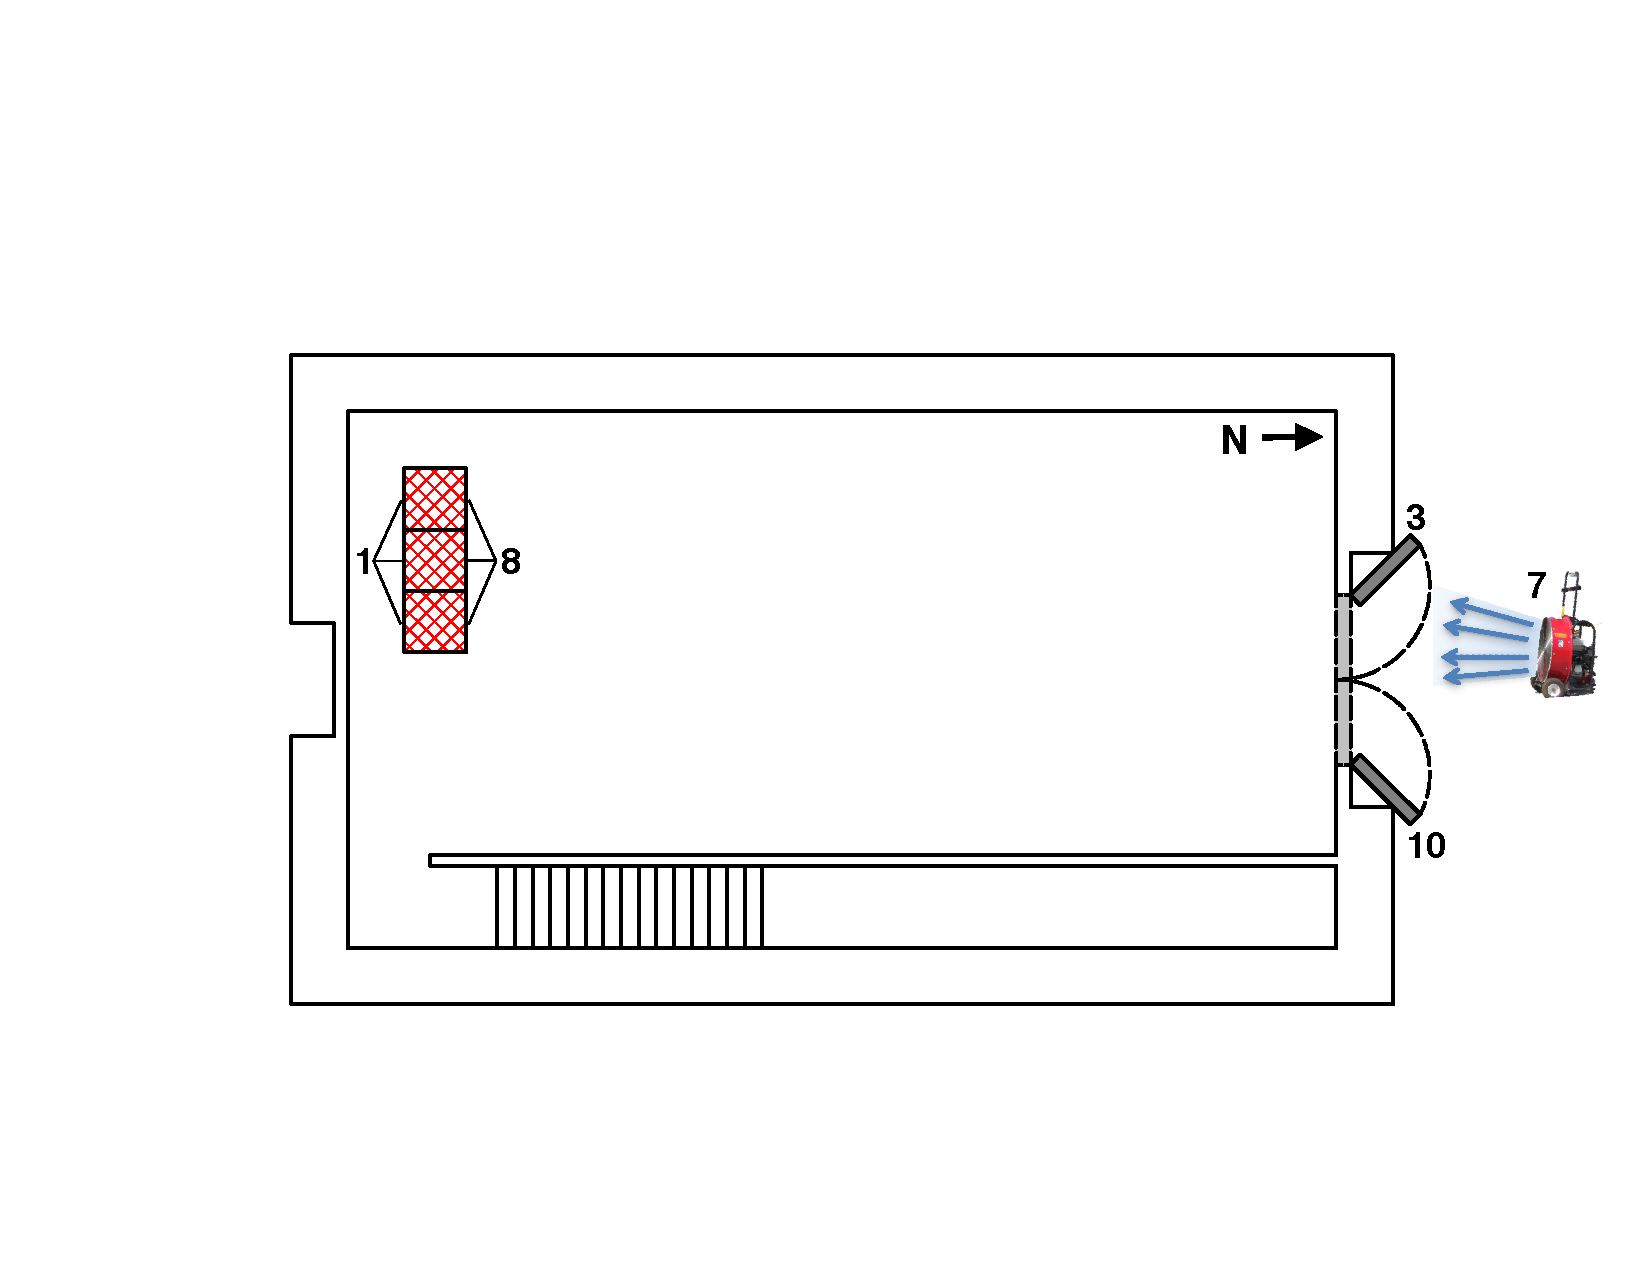
\includegraphics[width=0.95\columnwidth]{Figures/Floor_Plans/West_Structure_1st_Floor_Test_24}
\end{minipage}
\renewcommand{\baselinestretch}{1}
\caption{Tests 24--25 layout and event times.}
\label{fig:west_test_24}
\end{figure}
\renewcommand{\baselinestretch}{2}
\FloatBarrier
